%\documentclass[11pt,onecolumn,oneside]{article}
\documentclass{hitec}
%\usepackage[T1]{fontenc}
%\usepackage{lmodern}
\usepackage{epsf,pstricks,pst-grad,color}
\usepackage{cleveref}
\usepackage{graphicx,amssymb,amsmath,makeidx,psfrag,subfigure}
\usepackage{authda14,sws,wasysym,epsfig}
\usepackage{longtable,rotating,latexsym,eso-pic}
\usepackage[colorlinks=true,citecolor=blue,linkcolor=blue,bookmarks=true,urlcolor=blue,hyperfootnotes=true,plainpages=false,pdfpagelabels=true,breaklinks=true]{hyperref} %create interal an click-on links
%\usepackage{breakurl}
\usepackage{tikz}
\usepackage{tikz-3dplot}
\usepackage{listings}

\usepackage{fancyvrb}

\makeatletter
\newread\pin@file
\newcounter{pinlineno}
\newcommand\pin@accu{}
\newcommand\pin@ext{pintmp}
% inputs #3, selecting only lines #1 to #2 (inclusive)
\newcommand*\partialinput [3] {%
	\IfFileExists{#3}{%
		\openin\pin@file #3
		% skip lines 1 to #1 (exclusive)
		\setcounter{pinlineno}{1}
		\@whilenum\value{pinlineno}<#1 \do{%
			\read\pin@file to\pin@line
			\stepcounter{pinlineno}%
		}
		% prepare reading lines #1 to #2 inclusive
		\addtocounter{pinlineno}{-1}
		\let\pin@accu\empty
		\begingroup
		\endlinechar\newlinechar
		\@whilenum\value{pinlineno}<#2 \do{%
			% use safe catcodes provided by e-TeX's \readline
			\readline\pin@file to\pin@line
			\edef\pin@accu{\pin@accu\pin@line}%
			\stepcounter{pinlineno}%
		}
		\closein\pin@file
		\expandafter\endgroup
		\scantokens\expandafter{\pin@accu}%
	}{%
		\errmessage{File `#3' doesn't exist!}%
	}%
}

\newenvironment{markdown}%
{\VerbatimEnvironment\begin{VerbatimOut}{tmp.markdown}}%
	{\end{VerbatimOut}%
	\immediate\write18{pandoc tmp.markdown -t latex -o tmp.tex}%
	\input{tmp.tex}}

%\usepackage{natbib}
%\lstset{breaklines=true}
%\usepackage{multirow}
\lstset{basicstyle=\bfseries}
\bibliographystyle{apalike}
\usepackage[english]{babel}
\providecommand{\tightlist}{%
	\setlength{\itemsep}{0pt}\setlength{\parskip}{0pt}}

\makeindex
%\selectlanguage{english}
%\parindent0em \parskip1.5ex plus0.5ex minus 0.5ex
%% -------------------------------------------------------------------
%
%%\geometry{a4paper, left=20 mm, right= 25mm, top=2.0cm, bottom=2.0 cm}
%
%\newcommand\BackgroundPicture{%
%   \put(0,-50){
%     \parbox[b][\paperheight]{\paperwidth}{
%       \vfill
%       \centering
%%       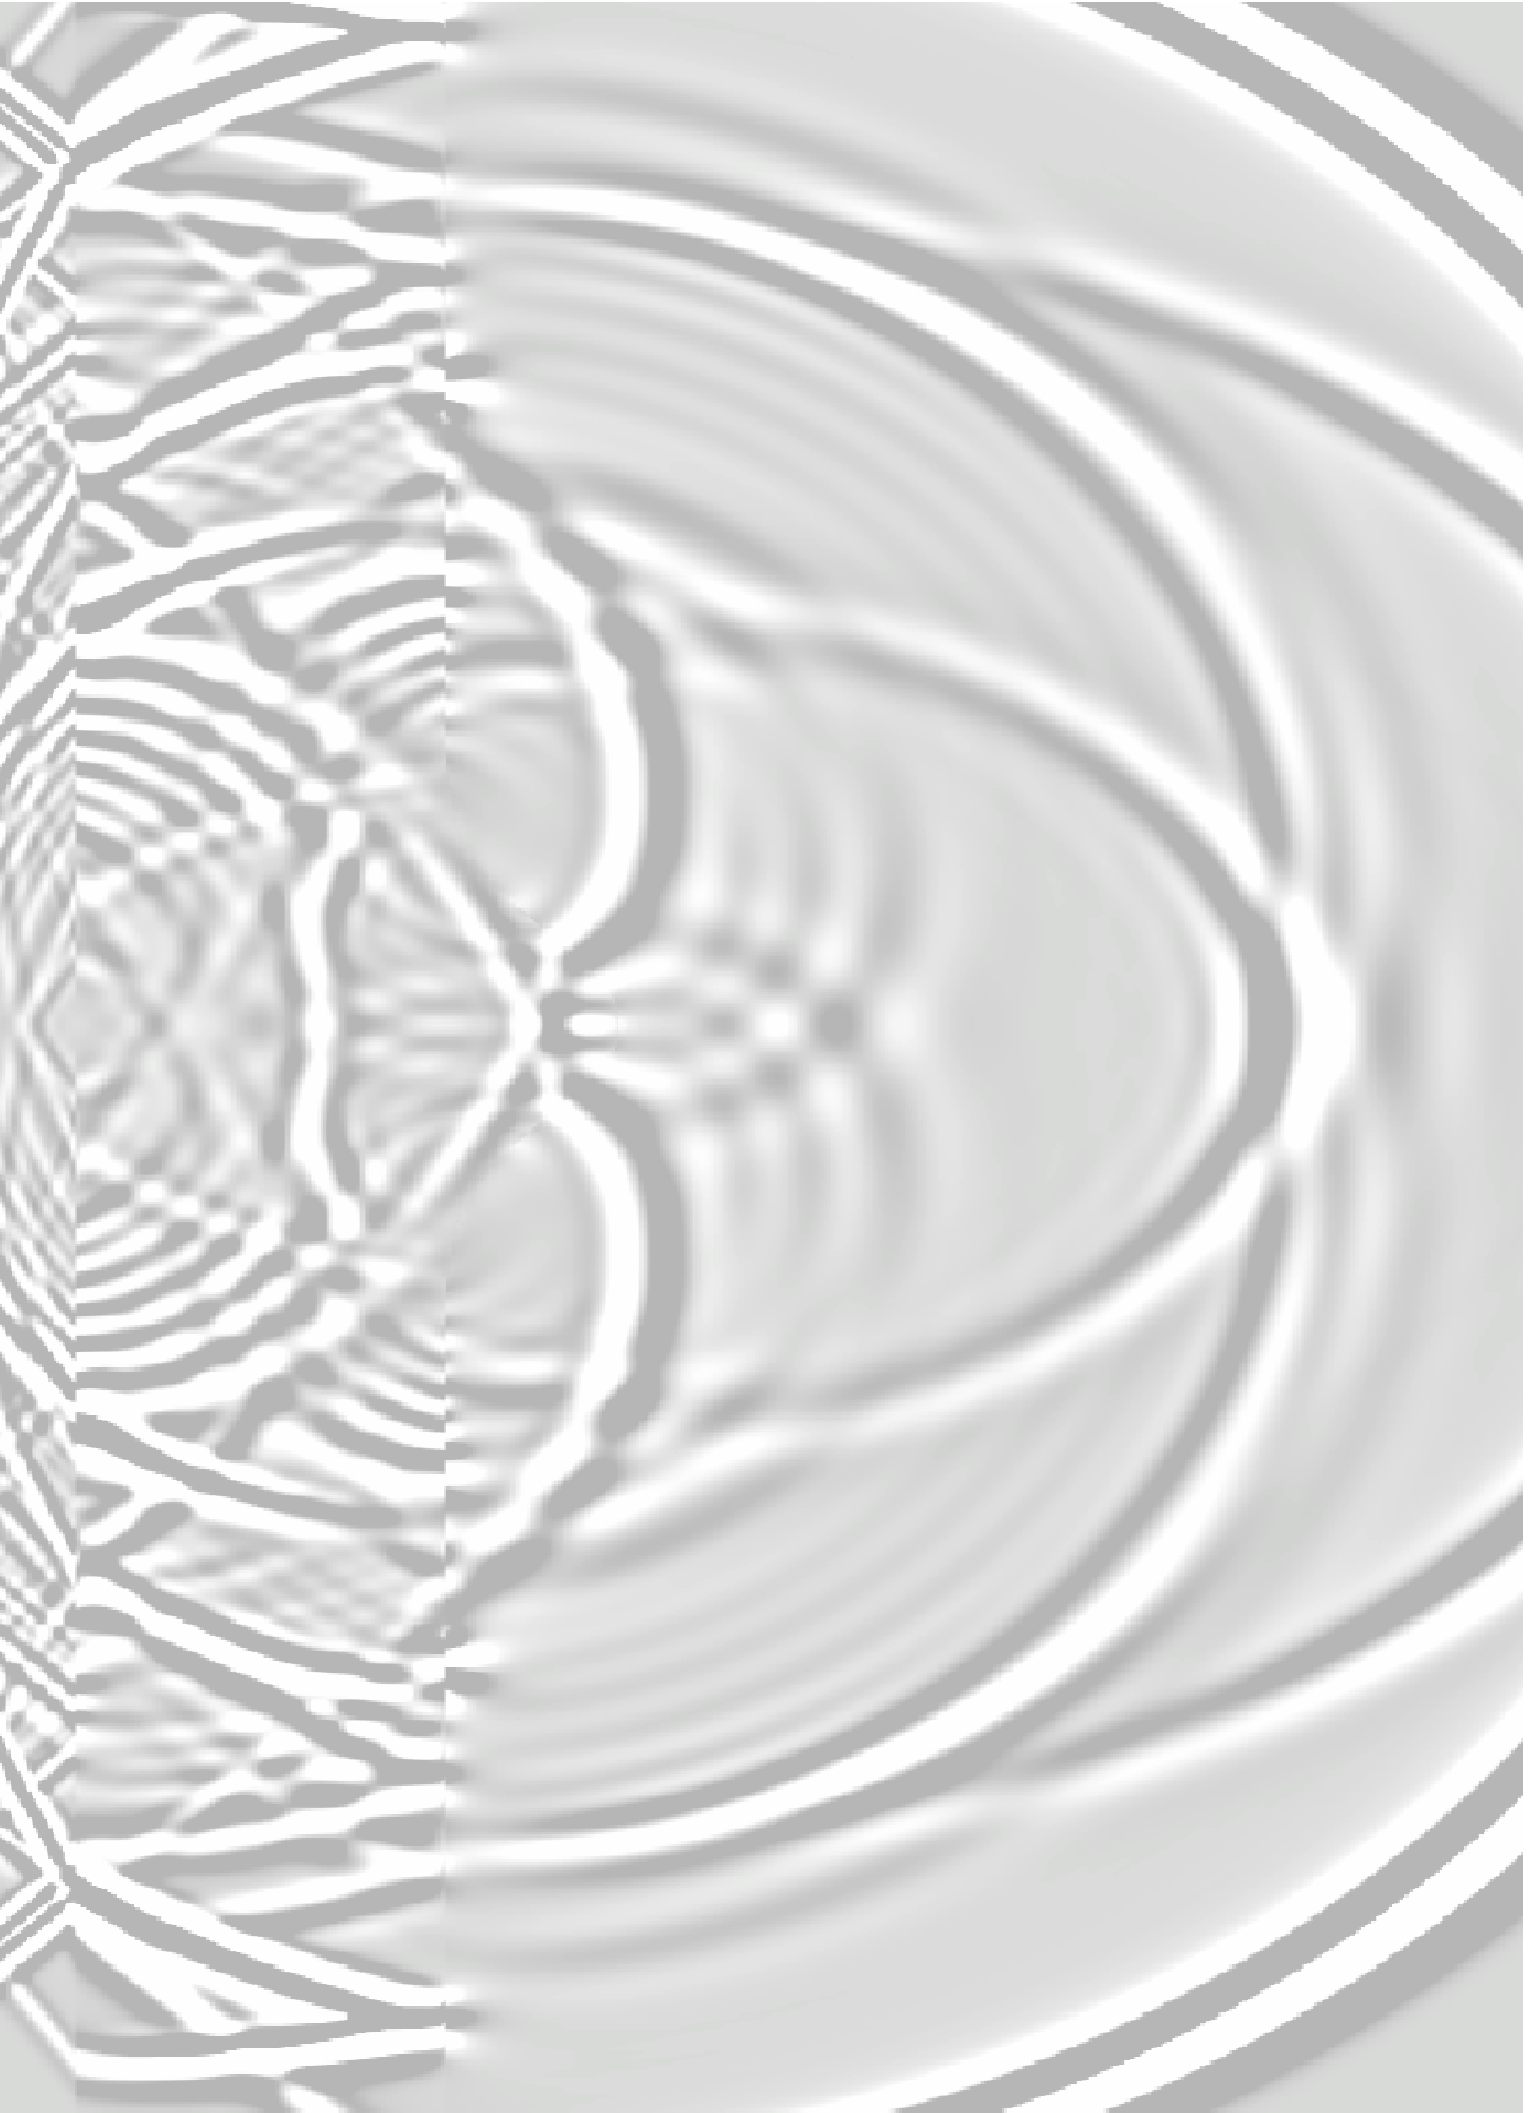
\includegraphics[width=\paperwidth,height=\paperheight,
%%                        keepaspectratio]{eps/title_page1.ps}
%
%       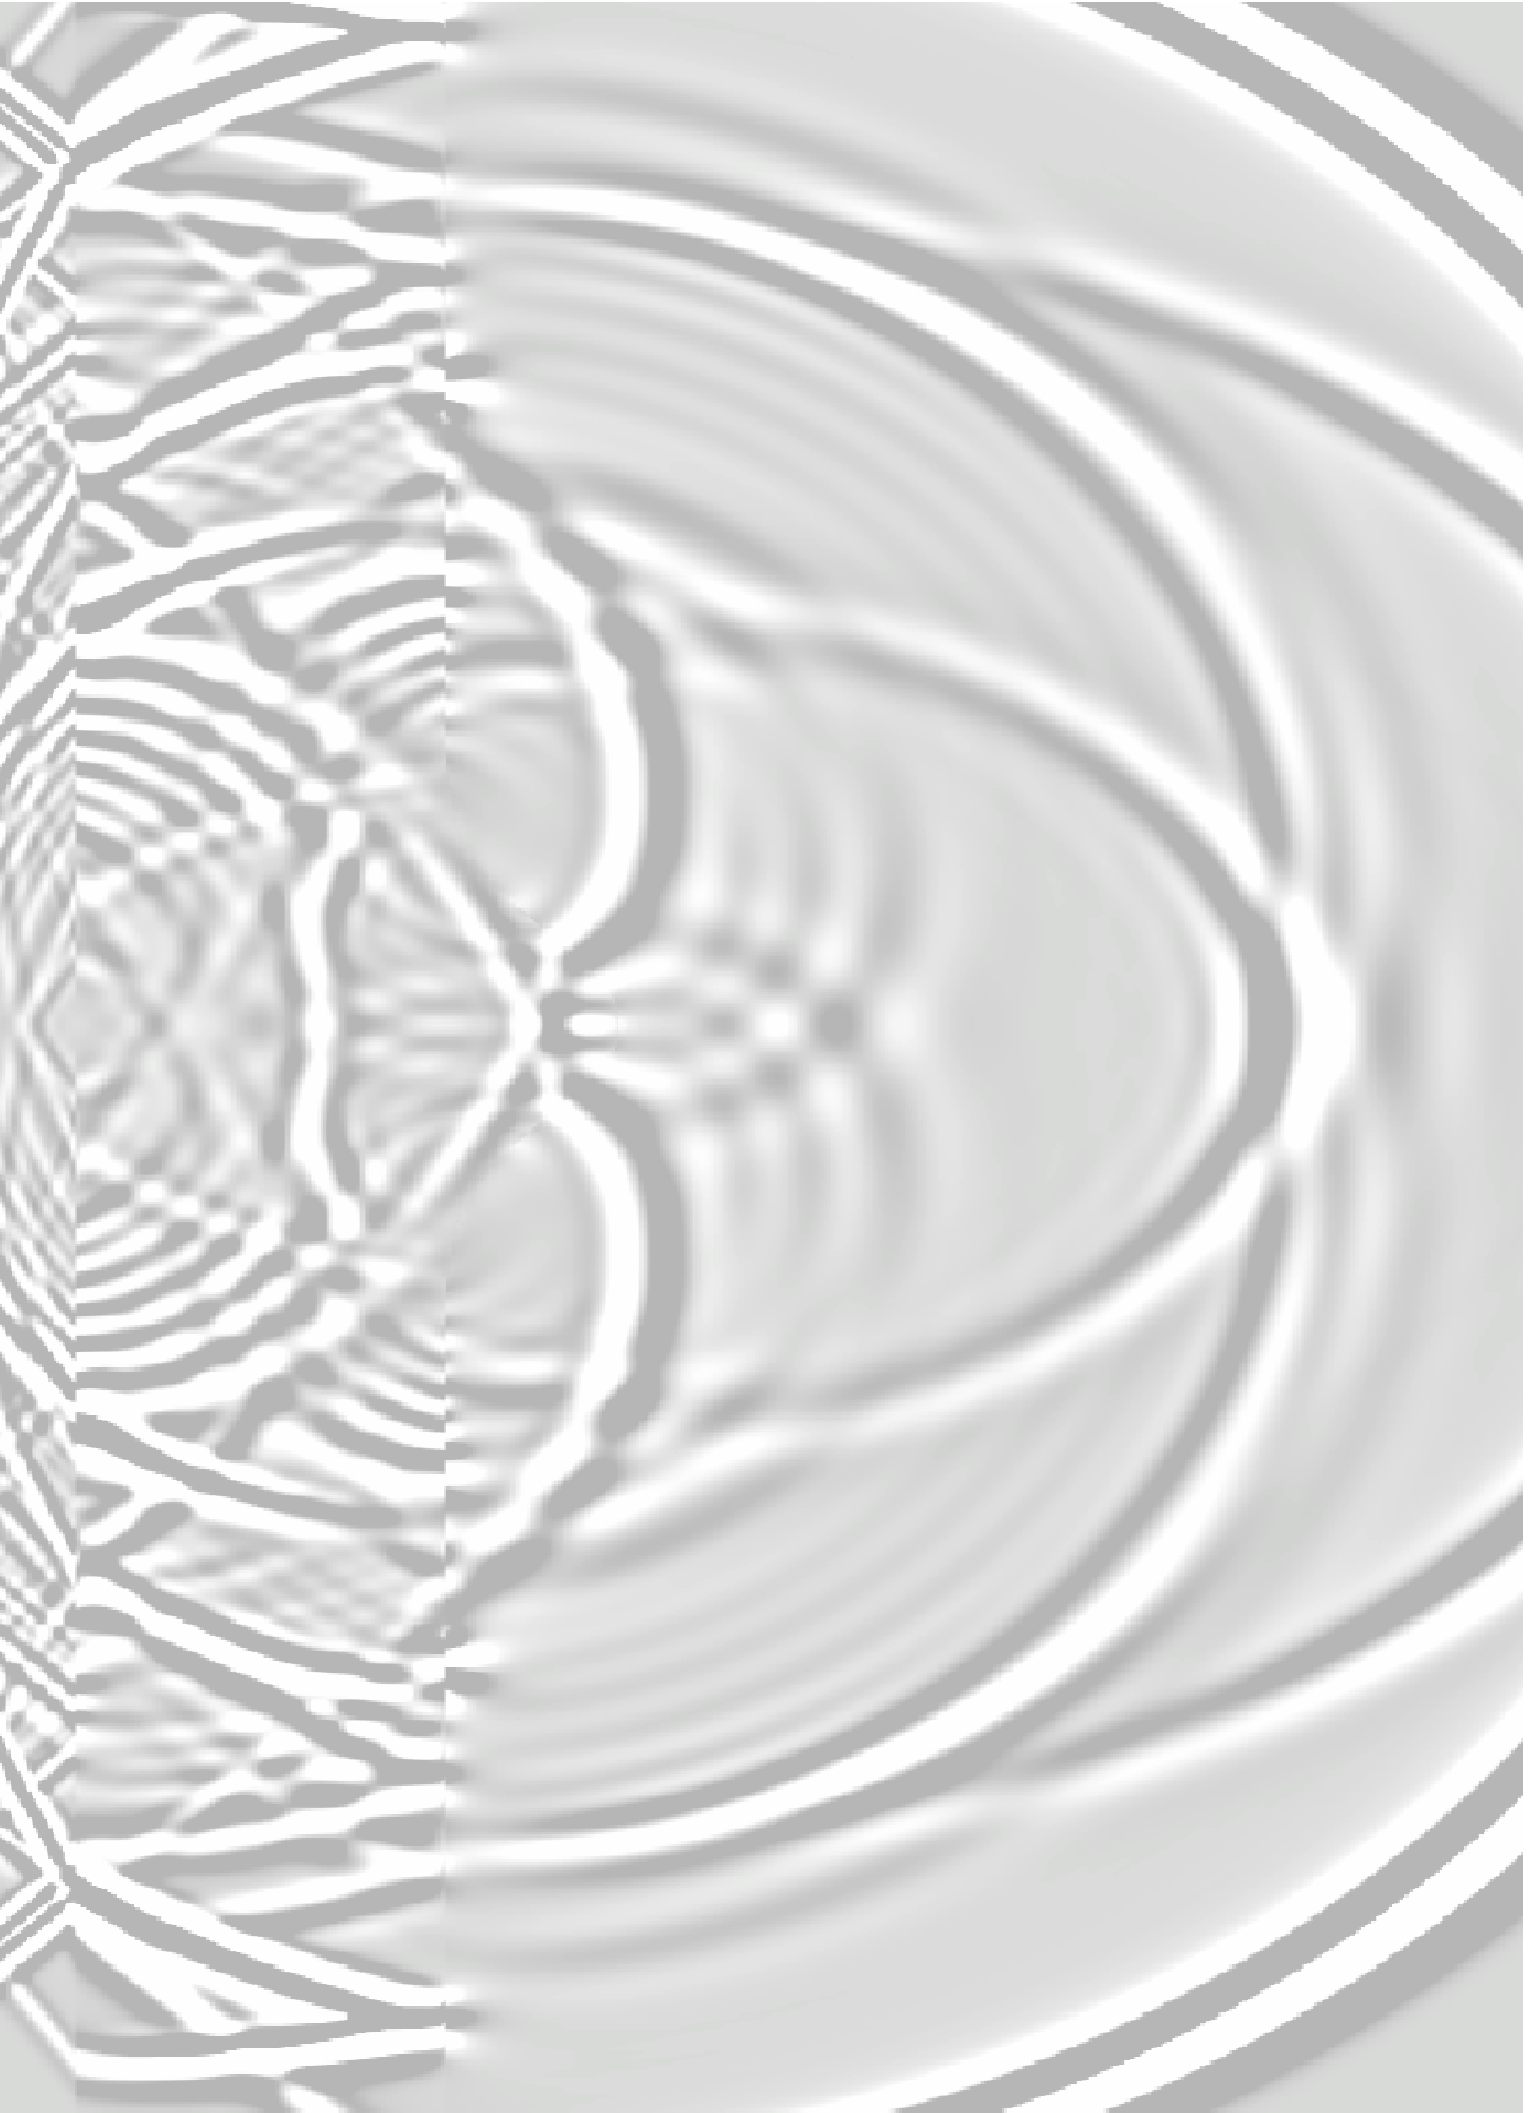
\includegraphics[width=\paperwidth,height=30cm]{eps/title_page1.pdf}
%       \vfill
%     }}}
%% The picture is centered on the page background
%% -------------------------------------------------------------------
%
%% add background picture for the titlepage
%
%% with this we ensure that the chapter and section 
%% headings are in lowercase 
%%\renewcommand{\chaptermark}[1]{markboth{#1}{}} 
%\renewcommand{\sectionmark}[1]{\markright{\thesection\ #1}} 
%\fancyhf{} %delete the current section for header and footer 
%\fancyhead[L,RO]{\bfseries\thepage}
%%\fancyhead[LE,RO]{\bfseries\thepage}  
%\fancyhead[LO]{\bfseries\rightmark} 
%%\fancyhead[RE]{\bfseries\leftmark}
%\fancyhead[R]{\bfseries\leftmark}  
%\renewcommand{\headrulewidth}{0.5pt}
% % make space for the rule 
%\fancypagestyle{plain}{% 
% \fancyhead{} %get rid of the headers on plain pages 
% \renewcommand{\headrulewidth}{0} % and the line 
%}
%
\newcommand{\option}[1]{\texttt{#1}}


\title{ASOFI anisotropic elastic seismic modeling with finite differences}
\author{Vladimir Kazei \& Dmitry Kabanov}

\begin{document}
	
\maketitle
ASOFI3D stands for Anisotropic Seismic mOdeling with FInite differences.
This code is a modification of
\href{https://git.scc.kit.edu/GPIAG-Software/SOFI3D/wikis/home}{SOFI3D}
to accomodate orthorhombic anisotropy

\tableofcontents

\section{Introduction}\label{intro}
In order to extract information about the structure and composition of the crust from seismic observations, it is necessary to be able to predict how seismic wavefields are affected by complex structures.
Since exact analytical solutions to the wave equations do not exist for most subsurface configurations, the solutions can be obtained only by numerical methods. For iterative calculations of synthetic seismograms with limited computer resources fast and accurate modeling methods are needed. 

The FD modeling program SOFI3D, that is described in this guide, is based on the FD approach described by \cite{virieux:86} and \cite{levander:88}. The present program SOFI3D has the following extensions

\begin{itemize}
	\item considers viscoelastic wave propagation effects like attenuation and dispersion \\
	\cite{robertsson:94,blanch:95,bohlen:02},
	\item employs higher order FD operators,
	\item applies Perfectly Matched Layer boundary conditions at the edges of the numerical mesh \cite{komatitsch:07},
	\item works in MPI parallel environment ONLY, i.e. SOFI3D is a implementation based on a domain decomposition
	\cite{bohlen:02}.
\end{itemize}

\subsection{License}\label{license}

ASOFI3D is free software: you can redistribute it and/or modify it under the terms of the GNU General Public License as published by the Free Software Foundation, version 2.0 of the License only.

ASOFI3D is distributed in the hope that it will be useful, but WITHOUT ANY WARRANTY; without even the implied warranty of MERCHANTABILITY or FITNESS FOR A PARTICULAR PURPOSE. See the GNU General Public License for more details. You should have received a copy of the GNU General Public License along with SOFI3D. See file COPYING and/or  \lstinline{http://www.gnu.org/licenses/gpl-2.0.html}.

The authors of ASOFI3D are listed in file  \lstinline{AUTHORS}.

%\newpage
\subsection{Requirements}
\label{requirements}

ASOFI3D has been tested under Linux \& Mac-OS. The preferred platform is Linux, since most of the large scale cluster computer run under Linux. On KAUST local workstations we use Ubuntu and OpenMPI.

\begin{center}
% use packages: array
\begin{small}
\begin{tabular}{lll}
Program & Description & Weblink \\ 
OpenMPI & MPI Implementation & \url{http://www.open-mpi.org} \\
 & (for the parallelization) & \\
C-Compiler & the whole code is written in C,& \\
& any C-Compiler should be able & \\
& to compile it & \\
Seismic Un*x & Seismic processing package, & \url{http://www.cwp.mines.edu/cwpcodes} \\
(SU)  & SOFI3D outputs seismic data & \\
& in the SU format & \\
Matlab & Preferred program package for & \url{http://www.mathworks.de} \\
(commercial)& the visualization of snapshots, also  & \\
& useful for the display and & \\
& processing of seismograms & \\
xmovie & Console based movie program, can & usually included in Linux distribution\\
& be used for the quick display & otherwise install from repository\\
& of snapshot data  &
\end{tabular}
\end{small}
\end{center}

\newpage 
\section{Quick start}\label{qguide}
%\begin{markdown}
%	\subsection{Obtaining the code}\label{obtaining-the-code}

Get the code from this repo:

\begin{verbatim}
git clone git@github.com:swag-kaust/TD.git
\end{verbatim}

Then switch to the cloned repo directory:

\begin{verbatim}
cd TD
\end{verbatim}

\subsection{Building the code}\label{building-the-code}

The prerequisites for ASOFI3D are:

\begin{itemize}
\tightlist
\item
  C compiler (for example, \texttt{gcc})
\item
  MPI library (for example, \href{https://www.open-mpi.org/}{OpenMPI})
\item
  Make build system (GNU Make is a popular choice)
\end{itemize}

\subsection{Compile with gcc and OpenMPI on
Ubuntu}\label{compile-with-gcc-and-openmpi-on-ubuntu}

On recent Ubuntu versions such as 14.04, 16.04, or 18.04 all
prerequisites can be obtained by the following commands:

\begin{verbatim}
sudo apt-get install gcc make libopenmpi-dev
\end{verbatim}

Then while in the root directory of the code, build the code via command

\begin{verbatim}
make
\end{verbatim}

which compiles the solver and several auxiliary utilities.

\subsection{Example usage}\label{example-usage}

After successful compilation, you can run the code via command

\begin{verbatim}
./run_ASOFI3D.sh np dirname
\end{verbatim}

where \texttt{np} is a number of MPI processes you want to use and
\texttt{dirname} is the directory that contains configuration of the
problem to solve. Parameter \texttt{dirname} is optional and defaults to
\texttt{par}, so that the main configuration file of the solver is
\texttt{par/in\_and\_out/sofi3D.json}.

\subsection{Running the tests}\label{running-the-tests}

To run the tests, Madagascar is an additional prerequisite. Tests are
run via the command

\begin{verbatim}
make test
\end{verbatim}

%\end{markdown}
\partialinput{12}{79}{README}

You may also use the shell script  \lstinline{startSOFI3D.sh} located in  \lstinline{sofi3D/par} that also writes the screen output to the file  \lstinline{sofi3D/par/in_and_out/sofi3D.jout}.

The modeling parameters are specified in the input file \lstinline{par/in_and_out/sofi3D.json}. The parameters should be more or less self-explanatory. The synthetic seismograms and snapshots are written to the files specified in the sofi3D input file. Model is generated on the fly by the function sofi3D/src/model\_elastic.c. This function generates a homogeneous medium with $v_p$=3500 m/s, $v_s$=2000 m/s, and $\rho$=2000 kg/$\mathrm{m}^3$. Instead, the function readmod.c can be used to read model info from external grid files. See readmod.c for the format of the external files. You can change the function which generates the model grid by switching the READMOD parameter in the sofi3D input file.

\subsection{Structure of the code}
\label{installation}
In the SOFI3D directory you will find different subdirectories:

\textbf{bin}\\
This directory contains all executable programs, generally sofi3D and snapmerge. These executables are generated using the command  \lstinline{make <program>} (see below).

\textbf{doc}\\
This directory contains documentation on the software (this users guide).

\textbf{src}\\
This directory contains the complete source codes.  The following programs are available and my be compiled using \lstinline{make <program>}.

\textbf{src/model\_elastic\_examples}\\
Contains the model and benchmark files for SOFI3D.

\textbf{mfiles}\\
Here some Matlab routines (m-files) are stored. 

\textbf{par}\\
Parameter files for SOFI3D modeling.

                       
\newpage

\section{Solving the Elastic Wave Equation}

\subsection{Anisotropic elastic Wave Equations}
After a short calculation we get the following system of linear 1st order differential equations: 

\EQ{1:15}{\rho \frac{dv_i}{dt} + v_i \rho \MB{\nabla} v_i = - \frac{\partial \sigma_{ij}}{\partial x_j} + f_i.}

The momentum equation is satisfied for any volume, independently if it is filled with a liquid, a gas or rock. For an {\bf{elastic medium}} exists a linear relationship between stress and strain:

\begin{equation} \label{eq:stressStrain}
\sigma_{ij}= c_{ijkl} \varepsilon_{kl},
\end{equation}

where $c_{ijkl}$ is the elasticity tensor, and
\begin{equation}
\varepsilon_{ij}=\biggl(\frac{\partial u_i}{\partial x_j}+\frac{\partial u_j}{\partial x_i}\biggr)\
\end{equation}
is the deformation or strain tensor.

The general elasticity tensor has symmetries:
\begin{equation}
c_{ijkl} = c_{jikl},~ and ~ c_{ijkl} = c_{klij}.
\end{equation}
Therefore it can be compactly written down in Voigt $(C_{ij}$ notation as a 6x6 matrix:
\begin{equation}
c_{ijkl} \equiv C_{N(i,j), N(k,l)},
\end{equation}
where
\begin{eqnarray}
N(i,i) = i, //
N(2,3) = 4,~ N(1,3) = 5, ~N(1,2) = 6.
\end{eqnarray}
In gneral anisotropic medium it leads the 21 elastic constants. We focus on orthorhombic medium which has nine non-zero elastic constants (Figure~\ref{fig:CijOrtho}, \cite{kazei2018}).

\begin{equation}
{\delta_{ij}=
	\begin{cases}
	1 & \text{for } i=j\\
	0 & \text{else}
	\end{cases} 
	\biggr \}: \;\text{Kronecker symbol} \notag}
\end{equation}

\begin{figure}
	\centering
	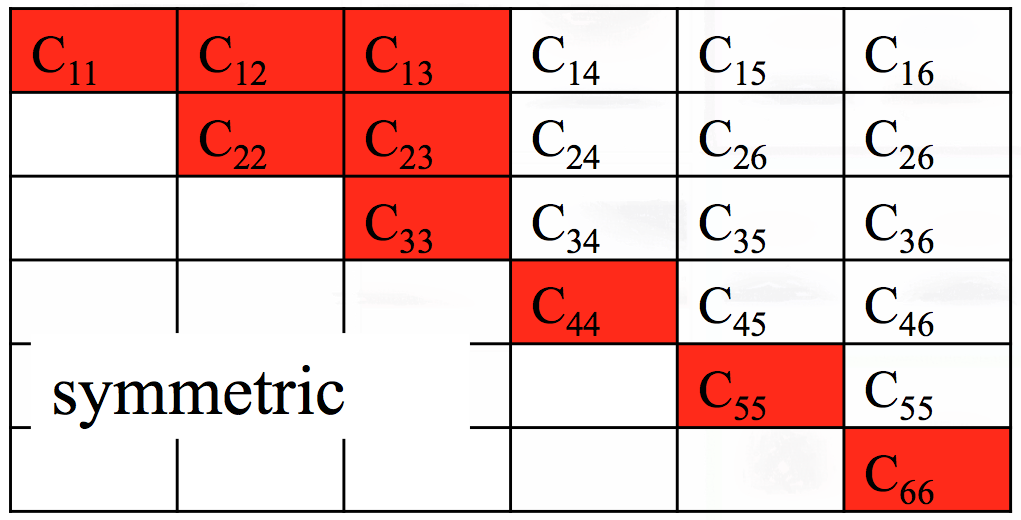
\includegraphics[width=0.5\linewidth]{eps/CijOrtho}
	\caption{Voigt notation for elasticity tensor, orthorhombic medium has only nine elastic parameters with non-zero values (in red).}
	\label{fig:CijOrtho}
\end{figure}

\subsection{Finite Differences}

To solve the equations \ER{1:15} and \eqref{eq:stressStrain} for an elastic medium, the particle velocities $\vec{v}$, the stresses $\sigma_{ij}$, the Lame parameters $\lambda$ and $\mu$ are calculated at  discrete cartesian coordinates  $x=i\; \times dx$, $y=j\; \times dy$, $z=k\; \times dz$ and at discrete times $t=n\; \times dt$ on a grid. $dx$, $dy$ and $dz$, denote  the spatial grid point distance in x-, y-, z-direction and $dt$ the difference between two succeeding time steps with $i \in N | [1,NX]$, $j \in N | [1,NY]$, $k \in N | [1,NZ]$ 
and $n \in N | [1,NT]$, where $NX$, $NY$, $NZ$ and $NT$ denote the number of spatial grid points and time steps. Finally the partial derivatives  are replaced by {\bf{(finite)-difference}} operators. The derivative of a function y after a variable x can be approximated by a forward $D^+$ or a backward operator $D^-$:

\EQ{disc:1}{\begin{split}
    D^+_x y&= \frac{y[i+1]-y[i]}{dh} \hspace{1 cm} \text{forward operator}\\
    D^-_x y&= \frac{y[i]-y[i-1]}{dh} \hspace{1 cm} \text{backward operator}\\
\end{split}}

To calculate with a larger grid point distance the variables are arranged on a staggered grid (\cite{virieux:86} and \cite{levander:88}) (Figure \ref{fig_cell}).  Please note, that the vertical axis is denoted by \textit{Y}, e.g. the indices of the stress components are labeled accordingly. To satisfy the stability of the {\bf{Standard Staggered Grid (SSG)}} code the density $\rho$, respectively. the Lame parameter $\mu$ are arithmetically and harmonically averaged (\cite{bohlen:06}):

\begin{figure}[ht]
\begin{center}
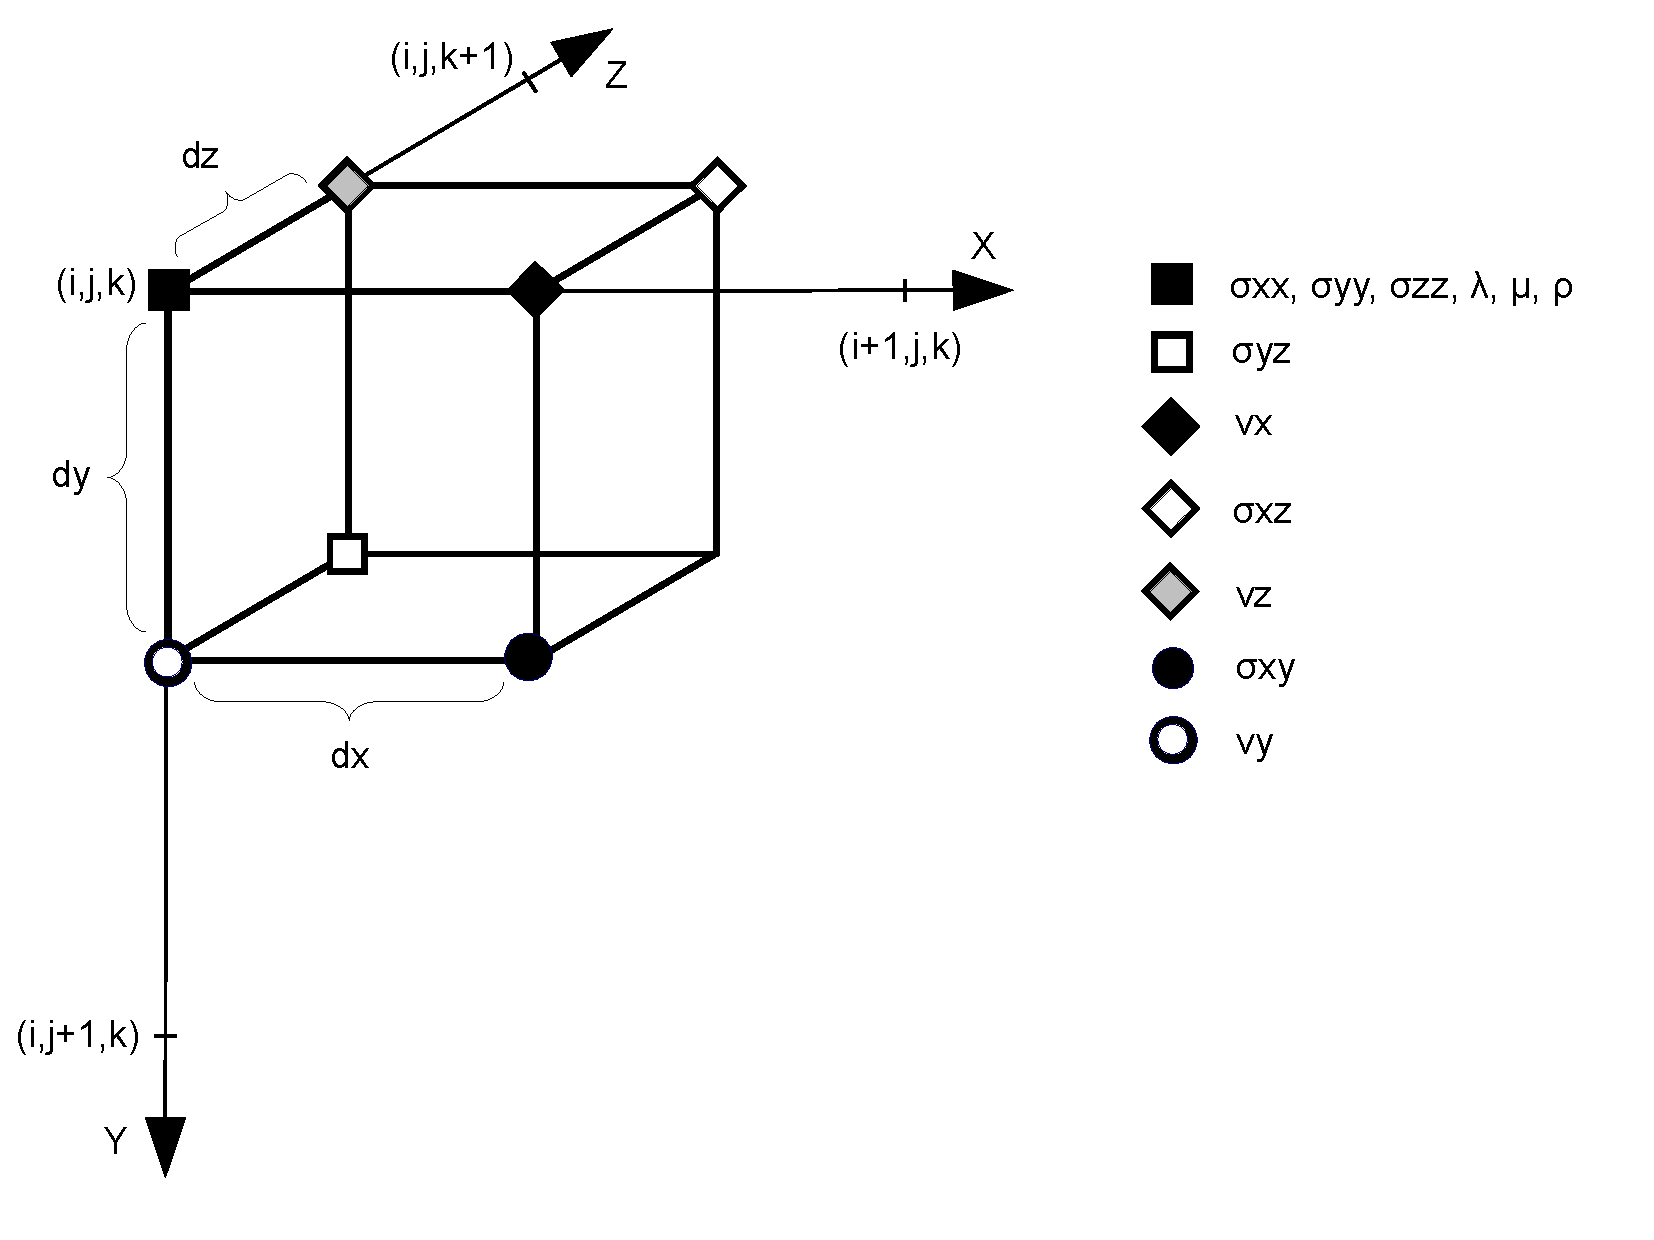
\epsfig{file=eps/ssg_grid.pdf, width=13 cm}
\caption{\label{fig_cell} Grid geometry for a Standard Staggered Grid (SSG).}
\end{center}
\end{figure}   




\newpage
\subsection{Accuracy of FD-operators}
In the previous section, the partial derivation was simply replaced by a finite difference quotient. In this section, a more systematical approach  is used. First the first derivation of the variable f at a grid point i is calculated using the following Taylor expansion:

\EQ{op_acc:1}{\begin{split}
    (2k-1)\frac{\partial f}{\partial x}\biggr|_i&=\frac{1}{dh}(f_{i+(k-1/2)}-f_{i-(k-1/2)})\\
    &+\frac{1}{dh}\sum_{l=2}^N \frac{(k-\frac{1}{2} dh)^{2l-1}}{(2l-1)!}\frac{\partial^{(2l-1)}f}{\partial
    x^{(2l-1)}}\biggr|_i+{\mathcal{O}}(dh)^{2N} \notag
\end{split}}

For an FD operator with length 2N N equations with a weighting factor $\beta_k$ are added:

\EQ{op_acc:2}{\begin{split}
    [\sum_{k=1}^{N} \beta_k (2k-1)]\frac{\partial f}{\partial x}\biggr|_i&=\frac{1}{dh} \sum_{k=1}^{N} \beta_k (f_{i+(k-1/2)}-f_{i-(k-1/2)})\\
    &+\frac{1}{dh}\sum_{k=1}^{N} \sum_{l=2}^N \beta_k \frac{(k-\frac{1}{2} dh)^{2l-1}}{(2l-1)!}\frac{\partial^{(2l-1)}f}{\partial
    x^{(2l-1)}}\biggr|_i+{\mathcal{O}}(dh)^{2N}
\end{split}}

For the case N=1 we get the FD operator from the previous section with length 2N=2. The Taylor series expansion will be aborted after the first  term (${\mathcal{O}}(dh)^{2}$). This operator is called {\bf{2nd order FD-operator}} which denotes the abortion error of the Taylor series and not the order of the desired approximated derivation. To understand equation \ER{op_acc:2} in more detail the coefficients for a {\bf{4th order FD-operator}} are calculated. The 4th order FD operator has the length 2N = 4, so N=2. By calculating the sums in \ER{op_acc:2} we get:

\EQ{op_acc:3}{\begin{split}
    (\beta_1+3 \beta_2) \frac{\partial f}{\partial x}\biggr|_i&=\frac{1}{dh}(\beta_1(f_{i-1/2}-f_{i+1/2})+\beta_2(f_{i-3/2}-f_{i+3/2}))\\
    &+\frac{dh^3}{dh}\biggl[\beta_1\frac{1}{8 \cdot 3!}+\beta_2\frac{27}{8 \cdot 3!}\biggr]\frac{\partial^3 f}{\partial x^3}\biggr|_i
\end{split}}

The weights $\beta_k$ are calculated in the following way:\\ 
The coefficients in front of the derivation on the LHS of Equation \ER{op_acc:3} should be equal to 1:

\EQ{op_acc:4}{(\beta_1+3\beta_2)=1 \notag.}

The coefficients before the derivation $\frac{\partial^3 f}{\partial x^3}\biggr|_i$ on the RHS of Equation \ER{op_acc:3} are vanishing:

\EQ{op_acc:5}{(\beta_1+27\beta_2)=0 \notag.}

The weighting coefficients $\beta_k$ can be calculated by inverting the following matrix equation:

\EQ{op_acc:6}{
\left(
\begin{array}{ll}
    1 & 3 \\
    1 & 27 \\
\end{array}
\right)\cdot \hspace{0.2 cm}
\left(
\begin{array}{l}
    \beta_1 \\
    \beta_2 \\
\end{array}
\right)
=
\left(
\begin{array}{l}
    1 \\
    0 \\
\end{array}
\right) \notag
}

The resulting coefficients are $\beta_1=9/8$ and $\beta_2=-1/24$, so the forward and backward 4th order FD operators look like:

\EQ{op_acc:7}{\begin{split}
    \frac{\partial f}{\partial x}\biggr|_{i+1/2}&=\frac{1}{dh}[\beta_1 (f_{i+1}-f_i)+\beta_2 (f_{i+2}-f_{i-1})] \hspace{1 cm} \text{forward operator}\\
    \frac{\partial f}{\partial x}\biggr|_{i-1/2}&=\frac{1}{dh}[\beta_1 (f_{i}-f_{i-1})+\beta_2 (f_{i+1}-f_{i-2})] \hspace{1 cm} \text{backward operator}\\
\end{split}}

The coefficients $\beta_i$ in the FD operator are called {\bf{Taylor coefficients}}. The accuracy of higher order FD operators can be improved significantly simply by slightly changes in the FD coefficients \cite{holberg:87}. These numerically optimized coefficients are called {\bf{Holberg coefficients}}.

\subsection{Grid Dispersion}\label{grid-dispersion}
The first question when building a FD model is: What is the maximum spatial grid point distance dh, for a correct sampling of the wavefield? To answer this question we take a look at this simple example: The particle displacement in x-direction is defined by a sine function:
\EQ{grid_disp:1}{v_x=\sin\biggl(2 \pi \frac{x}{\rm{\lambda}}\biggr),}
where $\rm{\lambda}$ denotes the wavelength. When calculating the derivation of this function analytically at $x=0$ and setting $\rm{\lambda}=1\;\rm{m}$ we get:
\EQ{grid_disp:2}{\frac{d v_x}{d x}\biggl|_{x=0}=\frac{2 \pi}{\rm{\lambda}} \cos\biggl(2 \pi \frac{x}{\rm{\lambda}}\biggr)\biggl|_{x=0}=2 \pi.}
In the next step the derivation is approximated numerically by a staggered 2nd order finite-difference operator:
\EQ{grid_disp:3}{\frac{d v_x}{d x}\biggl|_{x=0} \approx \frac{v_x(x+\frac{1}{2}\Delta x)-v_x(x-\frac{1}{2}\Delta x)}{\Delta x}\biggl|_{x=0}=\frac{\sin \biggl(\frac{2 \pi (\frac{1}{2}{\rm dx})}{\rm{\lambda}} \biggr)-\sin \biggl(\frac{2 \pi (\frac{1}{2}{\rm dx})}{\rm{\lambda}} \biggr)}{\Delta x}.}
Using the Nyquist-Shannon sampling theorem it should be sufficient to sample the wavefield with $\Delta x = \rm{\lambda}/2$. In table \ref{grid_disp.1} the
numerical solutions of eq. \ER{grid_disp:3} and the analytical solution \ER{grid_disp:2} are compared for different sample intervals 
$\Delta x = \rm{\lambda} /n$, where n is the number of gridpoints per wavelength. For the case n=2, which corresponds to the Nyquist-Shannon theorem, the
numerical solution is $\frac{d v_x}{d x}|_{x=0}=4.0$, which is not equal with the analytical solution $2 \pi$. A refinement of the spatial
sampling of the wavefield results in an improvement of the finite difference solution. For $\rm n=16$ the numerical solution is accurate to the second
decimal place. The effect of a sparsly sampled pressure field is illustrated in \FIG{grid_disp_pics} for a homogeneous block model with stress free surfaces. The dimensions of the FD grid are fixed
and the central frequency of the source signal is increased systematically. 
When using a spatial sampling of 16 grid points per minimum wavelength (\FIG{grid_disp_pics}, top) the wavefronts are sharply defined. For $\rm n=4$ 
grid points a slight numerical dispersion of the wave occurs (\FIG{grid_disp_pics}, center). This effect is obvious when using the Nyquist criterion ($\rm n=2$) 
(\FIG{grid_disp_pics}, bottom). Since the numerical calculated wavefield seem to be dispersive this numerical artefact is called {\bf{grid dispersion}}. 
To avoid the occurence of grid dispersion the following criteria for the spatial grid spacing dh has to be satisfied:
\EQ{grid_disp:4}{{\rm dh \le \frac{\lambda_{min}}{n}} = \frac{{\rm V_{min}}}{{\rm n}\; f_{max}}.}
Here $\rm{\lambda_{min}}$ denotes the minimum wavelength, $\rm{V_{min}}$ the minimum velocity in the model and $f_{max}$ is the maximum
frequency of the source signal.  
Depending on the accuracy of the used FD operator the parameter n is different.  In table \ref{grid_disp.2} n is listed for different FD operator lengths 
and types (Taylor and Holberg operators). The Holberg coefficients are calculated for a minimum dispersion error of $0.1\%$ at $3 f_{max}$. For short operators n should be choosen relatively large, so the spatial grid spacing is small, while for longer FD operators n is smaller and the grid spacing can be larger. 
\begin{table}[hbt]
	\begin{center}
		\begin{tabular}{ccc}\hline \hline
			n &  $\Delta x\; [m]$ & $\frac{d v_x}{d x}|_{x=0}\; []$ \\ \hline 
			analytical & - & $2\pi \approx 6.283$ \\ 
			2 & $\rm{\lambda}/2$ & 4.0 \\ 
			4 & $\rm{\lambda}/4$ & 5.657 \\ 
			8 & $\rm{\lambda}/8$ & 6.123 \\ 
			16 & $\rm{\lambda}/16$ & 6.2429 \\ 
			32 & $\rm{\lambda}/32$ & 6.2731\\ \hline \hline
		\end{tabular}
		\caption{\label{grid_disp.1} Comparison of the analytical solution Eq. \ER{grid_disp:2} with the numerical solution Eq. \ER{grid_disp:3} 
			for different grid spacings $\Delta x = \rm{\lambda /n}$.}
	\end{center}
\end{table}

\begin{table}[hbt]
	\begin{center}
		\begin{tabular}{ccc}\hline \hline
			FDORDER & n (Taylor) & n (Holberg) \\ \hline 
			2nd   &   12       &  12         \\
			4th   &   8        &  8.32       \\
			6th   &   6        &  4.77       \\
			8th   &   5        &  3.69       \\ 
			10th  &   5        &  3.19       \\
			12th  &   4        &  2.91       \\
			\hline \hline
		\end{tabular}
		\caption{\label{grid_disp.2} The number of grid points per minimum wavelength n for different orders (2nd-12th) and types (Taylor and
			Holberg) of FD operators. For the Holberg coefficients n is calculated for a minimum dispersion error of $0.1\%$ at $3 f_{max}$.}
	\end{center}
\end{table} 
\begin{figure}[ht]
	\begin{center}
		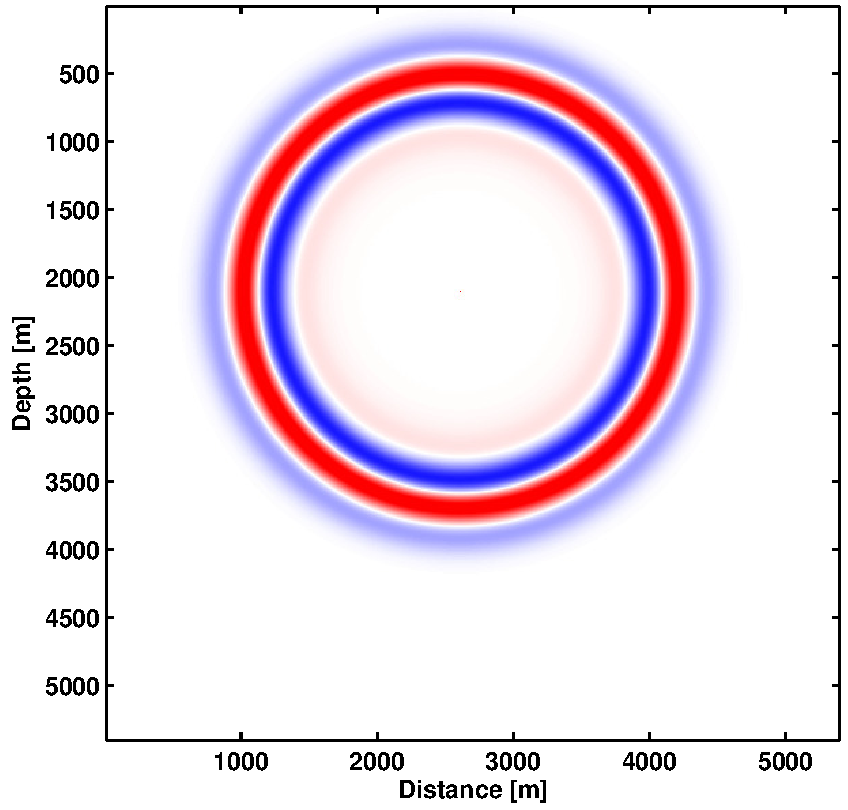
\epsfig{file=eps/homogenous_grid_n_16_5.pdf, width=4 cm}
		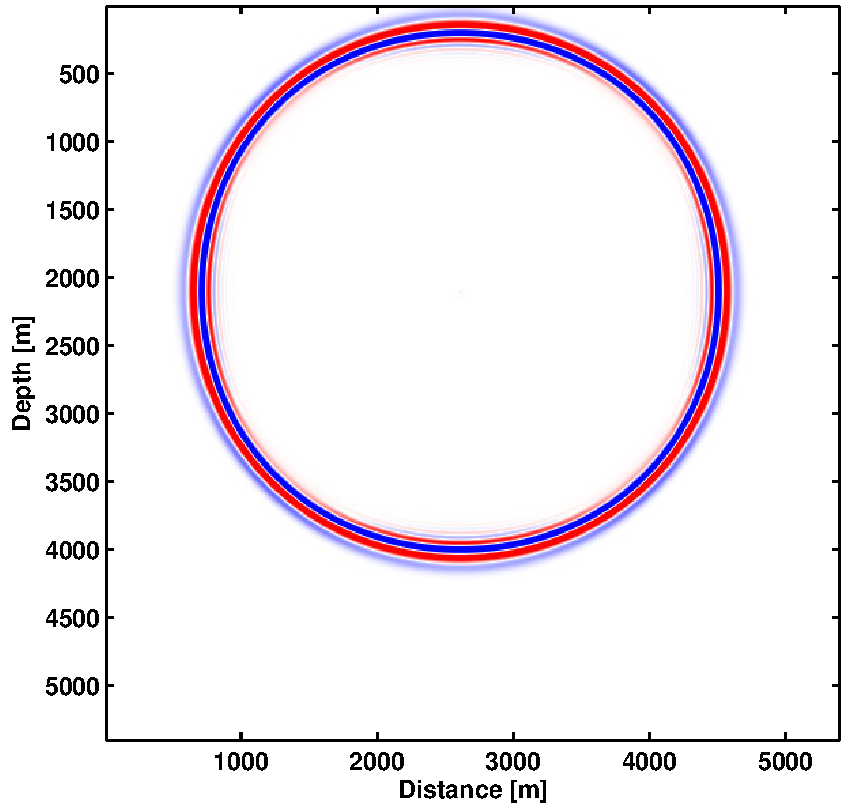
\epsfig{file=eps/homogenous_grid_n_4_5.pdf, width=4 cm}
		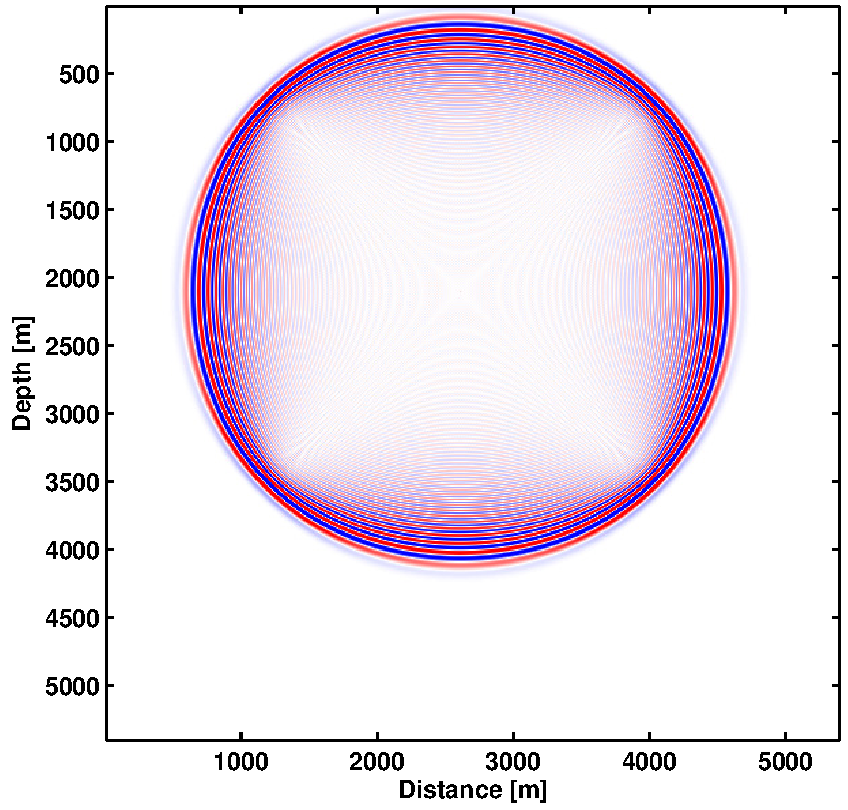
\epsfig{file=eps/homogenous_grid_n_2_5.pdf, width=4 cm}
		\caption{\label{grid_disp_pics} The influence of grid dispersion in FD modeling: Spatial sampling of the wavefield using n=16 (left), n=4 (center) and n=2 gridpoints (right) per minimum wavelength $\rm{\lambda_{min}}$.}
	\end{center}
\end{figure}
\clearpage
\subsection{The Courant Instability}\label{courant}
Beside the spatial, the temporal discretization has to satisfy a sampling criterion to ensure the stability of the FD code. If a 
wave is propagating on a discrete grid, then the timestep $dt$ has to be less than the time for the wave to travel between two adjacent grid 
points with grid spacing dh. For an elastic 2D grid this means mathematically:
\EQ{courant:1}{\rm{dt \le \frac{dh}{h \sqrt{2} V_{max}},}}
where $\rm{V_{max}}$ is the maximum velocity in the model. The factor h depends on the order of the FD operator and can easily calculated by summing over the weighting coefficients $\beta_i$
\EQ{courant:1:1}{{\rm{h} = \sum_i \beta_i.}}
In table \ref{courant.1} h is listed for different FD operator lengths and types (Taylor and Holberg operators). Criterion \ER{courant:1} 
is called {\bf{Courant-Friedrichs-Lewy criterion}} (\cite{courant:28}, \cite{courant:67}). When the Courant criterion is violated. After a few time steps the amplitudes are growing to infinity and the calculation becomes unstable, execution breaks.
\begin{table}[hbt]
	\begin{center}
		\begin{tabular}{ccc}\hline \hline
			FDORDER & h (Taylor)      & h (Holberg) \\ \hline 
			2nd   &   1.0             &  1.0        \\
			4th   &   7/6             &  1.184614   \\
			6th   &   149/120         &  1.283482   \\
			8th   &   2161/1680       &  1.345927   \\
			10th  &   53089/40320     &  1.387660   \\
			12th  &   1187803/887040  &  1.417065   \\   
			\hline \hline
		\end{tabular}
		\caption{\label{courant.1} The factor h in the Courant criterion for different orders (2nd-12th) and types (Taylor and Holberg) of FD operators.}
	\end{center}
\end{table} 

\newpage

\subsection{Boundary Conditions}\label{bound_cond}
To find to a unique solution of the problem, boundary conditions have to be defined. We can roughly distinguish two types of boundary conditions:

\begin{enumerate}

\item \underline{Dirichlet Boundary Conditions:}

The Dirichlet boundary condition specifies the values a solution needs to take on the boundary of a domain.
The Dirichlet boundary condition could take the form

\EQ{FD:5}{\begin{split}
    v_i(0)&=v_i(NX)=0 \\
    \sigma_{ij}(0)&=\sigma_{ij}(NX)=0
    \end{split}}

The Dirichlet boundary conditions have the disadvantage that it is not possible to model an infinite full space, because the wavefield is reflected at the boundaries of the model grid.

\item \underline{Absorbing Boundary Conditions:}

To overcome this disadvantage an absorbing boundary condition can be applied. A commonly used implementation is described in \cite{cerjan:85}: The numerical grid is enlarged by a few grid points ''$\rm{FW}$'' (typically $\rm{FW=30 gridpoints}$) in each direction. The values of the stress and particle velocity in this boundary frame are multiplied by a factor ''damp'':

\EQ{FD:5:1}{\rm{damp=exp(-a^2x^2)}}

with $\rm{a=\sqrt{-log(amp)/(FW)}}$ and $\rm{amp=0.92}$. The seismic waves are damped inside the boundary frame and cannot be reflected back into the model. This type of absorbing boundary
is not able to damp the reflected waves from the boundary completely.

A more effective way to damp the waves near the boundaries are the {\bf{Perfectly Matched Layers (PMLs)}}. This can be achieved by a coordinate stretch of the wave equations in the frequency domain \cite{komatitsch:07}. The coordinate stretch creates exponentially decaying plane wave solutions in the absorbing boundary frame. The PMLs are only reflectionless if the exact wave equation is solved. As soon as the problem is discretized (for example using finite differences) you are solving an approximate wave equation and the analytical perfection of the PML is no longer valid. To overcome this shortcoming the wavefield is damped by the damping function 

\EQ{FD:6:1}{\rm{c=-V_{pml} \cdot \frac{log(\alpha)}{L}}}

where $V_{pml}$ denotes the typical P-wave velocity of the medium in the absorbing boundary frame, $\alpha=1 \cdot 10^{-4}$ and L is the thickness of the absorbing boundary layer.

\end{enumerate} 
\clearpage





\section{Modeling Parameters}
\label{modelgeom}
The geometry of the FD grid and all parameters for the wave field simulation have to be defined in a parameter file (which we name in this case { \lstinline{sofi3D/par/in_and_out/asofi.json}}). In the following we will first list the full input file and later explain every input parameter section in detail:
\VerbatimInput{../../par/in_and_out/asofi.json}
All lines in the parameter file are formated according to the JSON standard (\url{http://www.json.org}) and organized as follows: 

\begin{verbatim}
"VARNAME" = "Parameter value",
\end{verbatim}

a comment line can look like this

\begin{verbatim}
"Comment" = "This is a useful comment",
"3D Grid information" = "comment",
\end{verbatim}

where VARNAME denotes the name of the global variable in which the value is saved in all functions of the program. The possible values are described in comments, feel free to add own comments. Basically all non JSON conform line will be ignored. The order of parameters can be arbitrary organized. The built-in JSON parser will search for the need parameters and displays found values. If critical parameters are missing the code will stop and an error message will appear. The meaning of the different parameters is described in the following.

\subsection{Coordinate system}
\label{coord_system}
ASOFI3D uses \textit{Y} as the vertical coordinate. All cooordinate related parameters read from the input file (such as DY and DZ, IDY and IDZ, REFREC,...) follow the logic that \textit{Y} denotes the depth (vertical axis).

Please note that if you choose the Seismic Unix output format ( \textbf{SEIS\_FORMAT = 1}) the coordinate orientation written into the header will not follow the SOFI3D coordinate convention as described above. Instead, the header word \textit{gy} denotes the second horizontal axis (equivalent to the \textit{Z} coordinate in SOFI3D) while the header word \textit{gelev} denotes the vertical axis (equivalent to the \textit{Y} coordinate in SOFI3D).


\subsection{Domain decomposition}

\begin{verbatim}
"Domain Decomposition" : "comment",
"NPROCX" : "2",
"NPROCY" : "2",
"NPROCZ" : "2",
\end{verbatim}

with

NPROCX : number of processors in x-direction\\
NPROCY : number of processors in y-direction\\
NPROCZ : number of processors in z-direction\\



Parallelization is based on domain decomposition (see Figure \ref{fig_grid}), i.e each processing element (PE) updates the wavefield within his portion of the grid. The model is  decomposed
by the program into sub grids. After decomposition each processing elements (PE) saves only his sub-volume of the grid. NPROCX, NPROCY and NPROCZ specify the number of
processors in x-, y- and z-direction, respectively (Figure  \ref{fig_grid}). The total number of processors thus is NP=NPROCX*NPROCY*NPROCZ. This value must be specified when starting the program with the mpirun command:  \lstinline{mpirun -np <NP> ../bin/sofi3D ./in_and_out/sofi3D.json} (see section \ref{compexec1}). If the total number of processors in sofi3D.json
and the command line differ, the program will terminate immediately with a corresponding error message (Try it !). Obviously, the total number of PEs (NPROCX*NPROCY*NPROCZ) used to decompose the model  should be less equal than the total number of CPUs which are available on your parallel machine. If you use LAM and decompose your model in more domains than CPUs are available two or more  domains will be updated on the same CPU (the program will not terminate and will produce the correct results). However, this is only efficient if more than one processor is available on each node. In order to reduce the amount of data that needs to be  exchanged between PEs, you should decompose the model into more or less cubic sub grids. In our example, we use 2 PEs in each direction: NPROCX=NPROCY=NPROCZ=2. The total number of PEs used by the program is NPROC=NPROCX*NPROCY*NPROCZ=8. 
\begin{figure}
\begin{center}
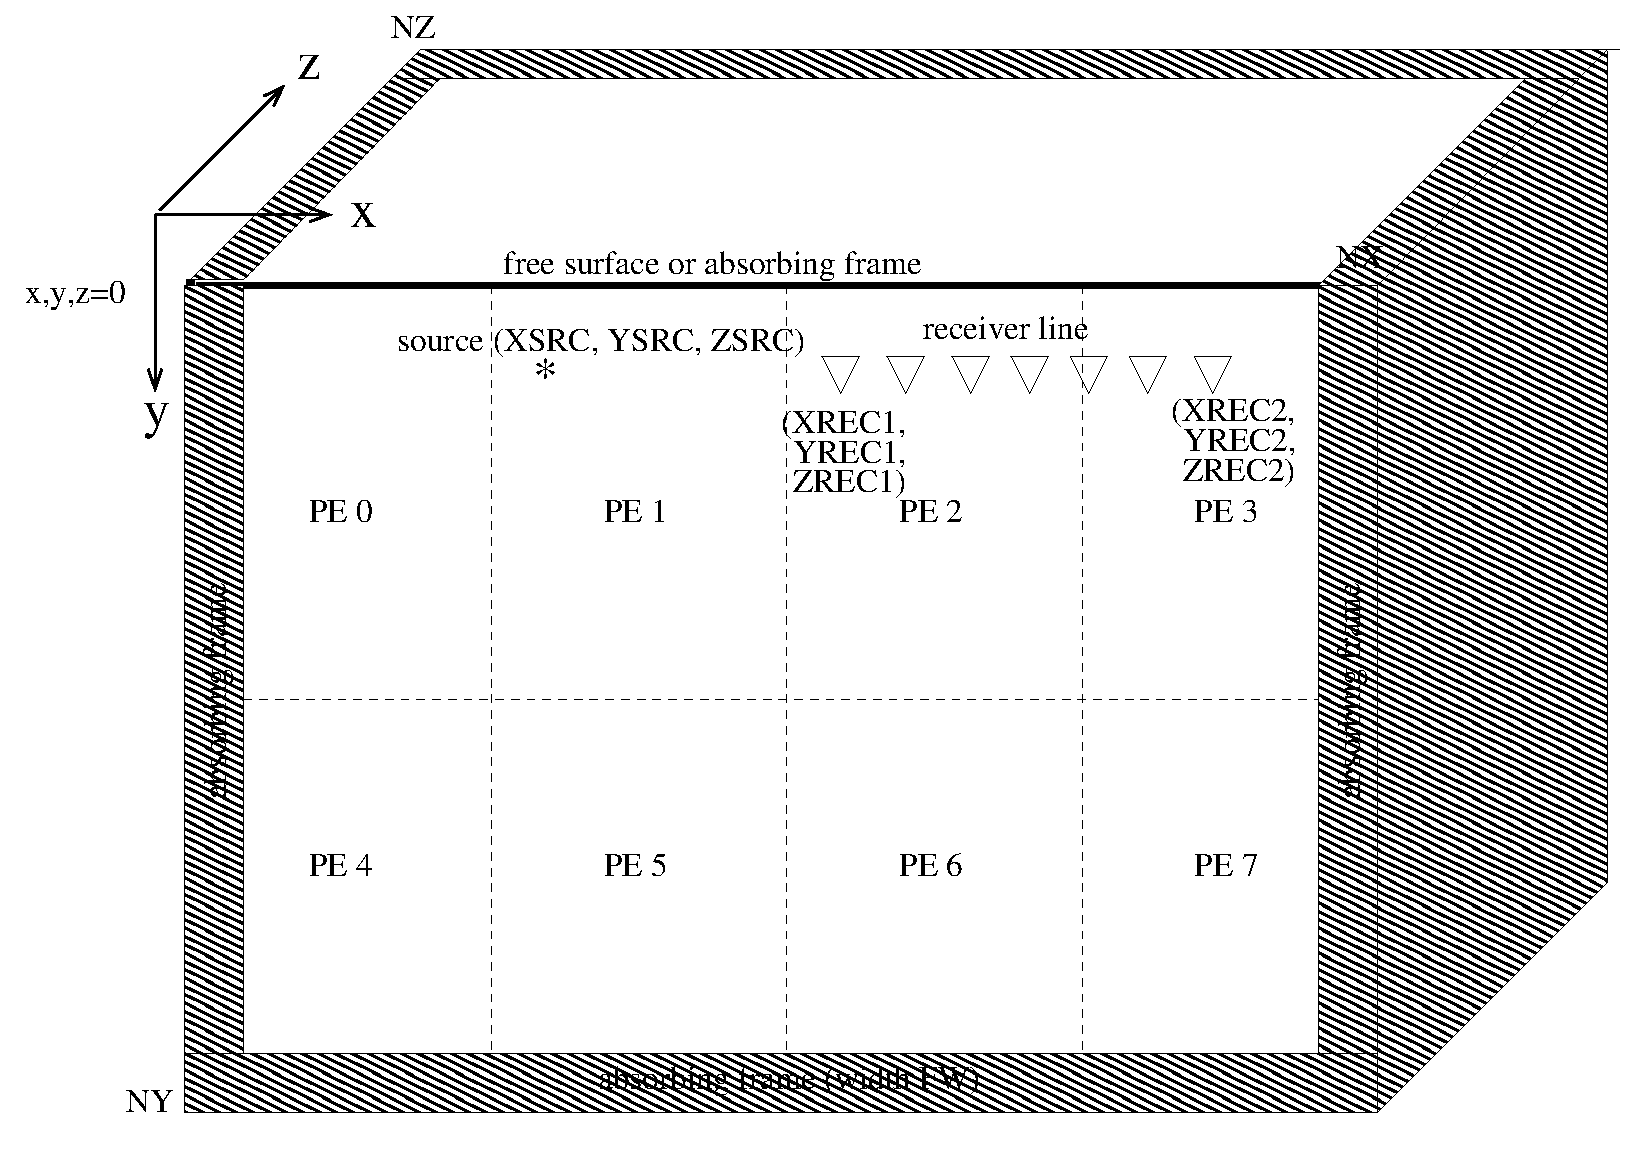
\includegraphics[width=\textwidth,angle=0]{eps/grid.pdf}
\end{center}
\caption{Geometry of the numerical FD grid using 4 processors in x-direction (NPROCX=4) and 2 processors in y-direction (NPROCY=2). Each processing element (PE) is updating the wavefield in his domain.
At the top of the numerical mesh the PEs apply a free surface boundary condition if FREE\_SURF=1, otherwise an absorbing boundary condition (ABS or PML) is applied. The width of the absorbing frame is FW grid points.  The size of the total grid is NX grid points in x-direction, NY gridpoints in y-direction and NZ gridpoints in z-direction. The size of each sub-grid  thus is NX/NPROCX x NY/NPROCY x NZ/NPROCZ gridpoints. The source is located at (XSRC,YSRC,ZSRC). The first receiver is at (XREC1,YREC1,ZREC1) and the  last receiver at (XREC2,YREC2,ZREC2). The origin of the Cartesian coordinate system (x,y,z) is at the top left corner of the grid. }
\label{fig_grid}
\end{figure}
\subsection{Discretization}
\begin{verbatim}
"3-D Grid" : "comment",
"NX" : "100",
"NY" : "100",
"NZ" : "100",
"DX" : "54.0",
"DY" : "54.0",
"DZ" : "54.0",
\end{verbatim}

with

NX : number of gridpoints in x-direction\\
NY : number of gridpoints in y-direction\\
NZ : number of gridpoints in z-direction\\
DX : distance between gridpoints(in m) in x-direction\\
DY : distance between gridpoints(in m) in y-direction\\
DZ : distance between gridpoints(in m) in z-direction\\
Caution: first gridpoint is not at {0.0,0.0,0.0} but at {dx,dy,dz}!\\
Note that Y denotes the vertical direction !\\


These lines specify the size of the total numerical grid (Figure  \ref{fig_grid}). NX, NY and NZ give the number of grid points in the x-, y- and z-direction, respectively, and DX, DY and DZ
specify the grid spacing in x-, y- and z-direction, respectively. The grid spacing may thus vary in the three directions to allow for a detailed discretization of small borehole tool features.
The size of the total internal grid in meters in x-direction is NX*DX, in y-direction NY*DY  and in z-direction NZ*DZ. To allow for a consistent domain decomposition NX/NPROCX, NY/NPROCY and NZ/NPROCZ must be integer values.

To avoid numerical dispersion the wavefield must be discretized with a certain number of gridpoints per wavelength. The number of gridpoints per wavelength required, depends on the order of the spatial
FD operators used in the simulation (see section \ref{grid-dispersion}). In the current FD software, 2nd, 4th, 6th, 8th, 10th and 12th order operators are implemented. The criterion to avoid numerical dispersion reads:
\begin{equation}
max(DX,DY,DZ)\le\frac{v_{s,min}}{2 f_c n} \label{eq_dispersion}
\end{equation}
where $\frac{v_{s,min}}{2 f_c}$ is the smallest wavelength propagating through the model. $v_{s,min}$ denotes the minimum shear wave velocity in the model, and $f_c=1/TS$ is the center frequency of the source wavelet. The program assumes that the maximum frequency of the source signal is approximately two times the center frequency. The center frequency is approximately one over the duration time TS. The value of n for different FD operators is tabulated in table \ref{grid_disp.2}. The criterion \ref{eq_dispersion} is checked by the FD software. If the criterion is violated a warning message will be displayed in the SOFI3D output (default :  \lstinline{./in_and_out/sofi3D.jout}), section ``--- CHECK FOR GRID DISPERSION ---``. Please note, that the FD-code will NOT terminate due to grid dispersion, only a warning is given in the output file.

\subsection{Order of the FD operator}

\begin{verbatim}
"FD order" : "comment",
"FDORDER" : "8",
"FDORDER_TIME" : "2",
"FDCOEFF" : "2",
\end{verbatim}

The order of the used spatial FD operator is defined by the option FDORDER. The possible values are 2, 4, 6, 8, 10, 12. 
The variable FDORDER\_TIME represents the used temporal FD order. FDORDER\_TIME=2 correspondents to the classical leapfrog scheme. Available higher order temporal FD operators are 3 and 4. Higher temporal orders will increase memory usage significant at least by a factor of 2.2. With the option FDCOEFF the user can switch between Taylor (FDCOEFF=1) and Holberg (FDCOEFF=2) FD coefficients. The chosen FD operator and FD coefficients have an influence on the numerical stability and grid dispersion (see section \ref{grid-dispersion}).


\subsection{Time stepping}
\begin{verbatim}
"Time Stepping" : "comment",
"TIME" : "5.0",
"DT" : "6.6e-3",
\end{verbatim}

with

TIME : time of wave propagation\\
DT : timestep (in seconds)\\


The propagation time of seismic waves in the entire model is TIME. The time stepping interval (DT) has to fulfill the stability criterion \ER{courant:1} in section \ref{courant}. 
The program checks these criteria for the entire model, outputs a warning message if these are violated , stops the program and will output the time step interval for a stable model run. 


\subsection{Sources}
\label{Sources}
\begin{verbatim}
"SOURCE_SHAPE" : "1",
"source shape values: ricker=1;fumue=2;from_SIGNAL_FILE=3;SIN**3=4" : "comment",
"SIGNAL_FILE" : "signal_mseis.tz",

"SOURCE_TYPE" : "1",
"source_type values (point_source):" : "comment",
"explosive=1;force_in_x=2;in_y=3;in_z=4;custom=5;double_couple=6" : "comment",
"SOURCE_ALPHA, SOURCE_BETA" : "0.0 , 0.0",
"AMON, STR, DIP, RAKE" : "1.0e2 , 45.0 , 90.0 , 45.0",
"SRCREC" : "1",
"srcrec values :  read from SOURCE_FILE=1, PLANE_WAVE=2 (internal)" : "comment"
            
"SOURCE_FILE" : "./sources/sources.dat", 
"RUN_MULTIPLE_SHOTS" : "0", 
            
"PLANE_WAVE_DEPTH" : "2106.0",
"PLANE_WAVE_ANGLE" : "0.0",
"TS" : "0.2",
\end{verbatim}

with

SOURCE\_SHAPE : Shape of source-signal (ricker=1, fumue=2, from SIGNAL\_FILE=3, SIN$^3$=4) \\
SOURCE\_TYPE : point source (explosive=1, force in x=2, in y=3, in z=4, custom=5, double couple=6) \\
If SOURCE\_TYPE $<$ 5 the SOURCE\_ALPHA and SOURCE\_BETA are ignored \\
SOURCE\_ALPHA : force angle between X and Z coordinate (in degree)\\
SOURCE\_BETA : force angle between:: Y and Z coordinate (in degree)\\
if SOURCE\_TYPE $\ne$ 6 the AMON, STR, DIP and RAKE are ignored\\
AMON: Seismic Moment of the earthquake (in newton meter)\\
STR: strike angle of the earthquake fault plane (in degree)\\
DIP: dip angle of the earthquake fault plane (in degree)\\
RAKE: rake angle of the slip vector (in degree)\\
PLANE\_WAVE\_DEPTH : depth of plane wave excitation (no$<$=0) (in meter)\\
if PLANE\_WAVE\_DEPTH$>$0, SRCREC is treated as 0\\
if PLANE\_WAVE\_DEPTH = 0 the PLANE\_WAVE\_ANGLE and TS  are ignored\\
PLANE\_WAVE\_ANGLE : dip of plane wave from vertical (in degrees)\\
TS : duration of source-signal (in seconds)\\
SIGNAL\_FILE : external signal file name \\
SRCREC : read source positions from SOURCE\_FILE (yes=1)\\
SOURCE\_FILE : external source file name \\
RUN\_MULTIPLE\_SHOTS : run multiple shots defined in SOURCE\_FILE (yes=1)\\
Note that Y denotes the vertical direction!\\

Three built-in wavelets of the seismic source are available. The corresponding time functions are defined in src/wavelet.c. You may modify the time functions in this file and recompile to include your
own analytical wavelet or to modify the shape of the built-in wavelets.

Ricker wavelet:
\begin{equation}
r(\tau)=\left(1-2\tau^2\right)\exp(-\tau^2) \quad \mbox{with} \quad \tau=\frac{\pi(t-1.5/f_c-t_d)}{1.0/f_c}
\label{eq_ricker}
\end{equation}

Fuchs-M\"uller wavelet:
\begin{equation}
f_m(t)=\sin(2\pi(t-t_d)f_c)-0.5\sin(4\pi(t-t_d)f_c) \quad \mbox{if} \quad t\in[t_d,t_d+1/fc] \quad \mbox{else} \quad fm(t)=0
\label{eq_fm}
\end{equation}

$sin^3$ wavelet:
\begin{equation}
s3(t)=0.75 \pi f_c \sin(\pi(t+t_d)f_c)^3\quad \mbox{if} \quad t \in[t_d,t_d+1/fc] \quad \mbox{else} \quad s3(t)=0
\label{eq_s3}
\end{equation}

In these equations, t denotes time and $f_c=1/TS$ is the center frequency. $t_d$ is a time delay which can be defined for each source position in SOURCE\_FILE. Variable time delays for different sources locations allow the simulation of passive acoustic emission. Note that the symmetric (zero phase) Ricker signal is always delayed by $1.0/f_c$, which means that after
one period the maximum amplitude is excited at the source location.  These three source wavelets and the corresponding amplitude spectra for a center frequency of $f_c=50$ Hz and
a delay of $t_d=0$ are plotted in Figure \ref{fig_source_wavelets}. Note the delay of the Ricker signal described above. The Fuchs-M\"uller wavelet has a slightly higher center frequency and covers a broader frequency range.

\begin{figure}
\begin{center}
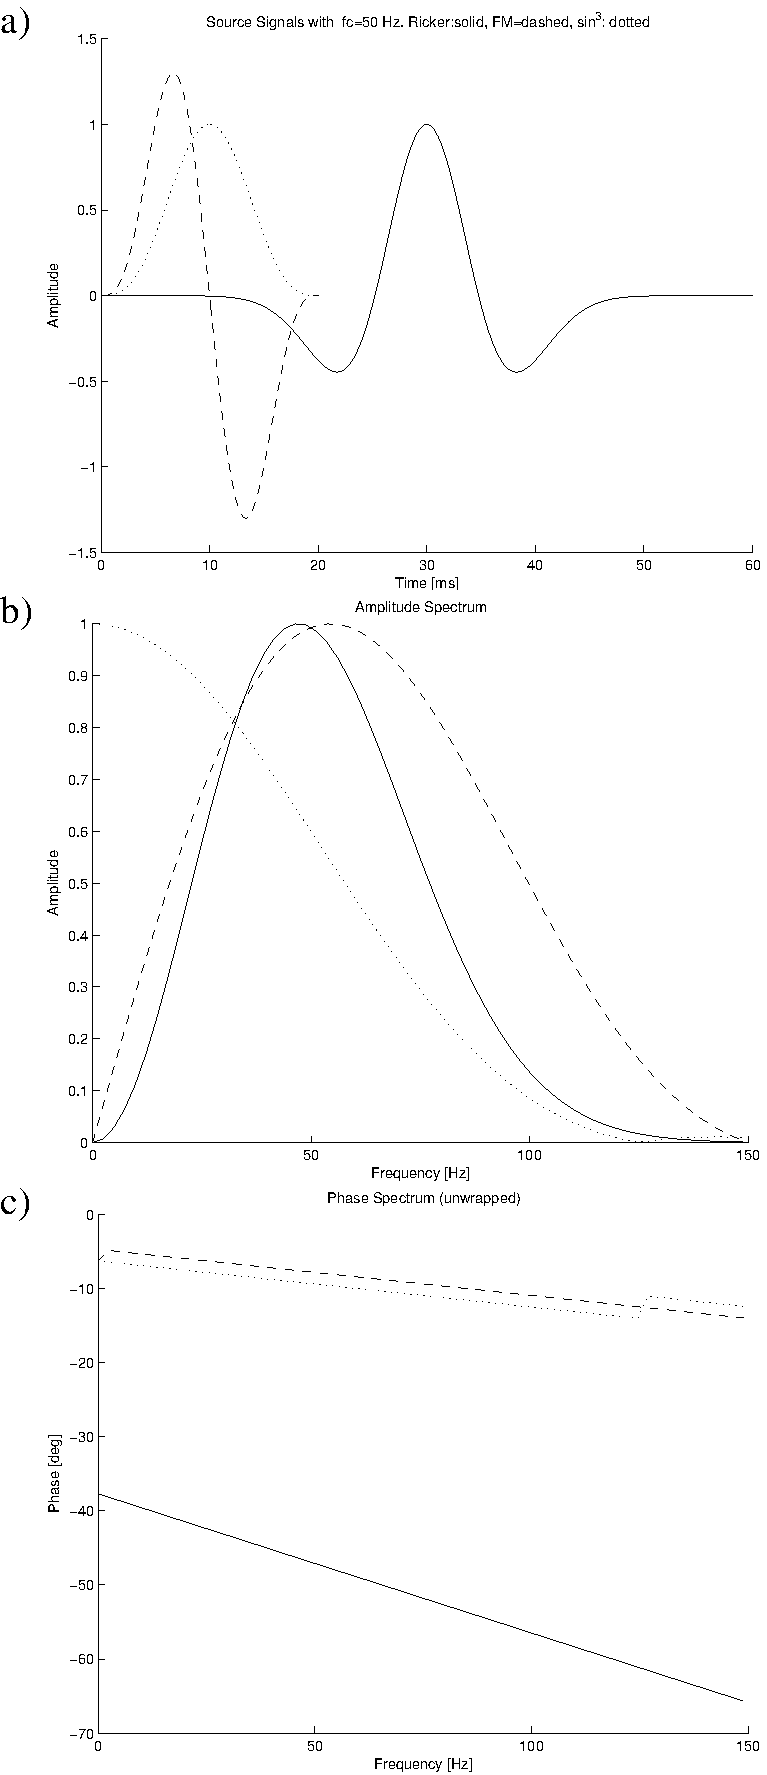
\includegraphics[width=7cm,angle=0]{eps/signals.pdf}
\end{center}
\caption{Plot of built-in source wavelets (equations \ref{eq_ricker}, \ref{eq_fm}, \ref{eq_s3}) for a center frequency of $f_c=50$ Hz 
($TS=1/f_c=0.02$s): Ricker signal (solid), Fuchs-M\"uller signal (dashed), $sin^3$-signal (dotted). a) Time function, b) amplitude
spectrum, c) phase spectrum.  }
\label{fig_source_wavelets}
\end{figure}

You may also use your own digitized time function as the source wavelet (for instance the signal of the first arrival recorded by a geophone at near offsets). Specify SOURCE\_SHAPE=3 and save the samples of
your source wavelet in ASCII-format in SIGNAL\_FILE. SIGNAL\_FILE should contain one sample per line. It should thus look like:

\begin{verbatim}
0.0
0.01
0.03
...
\end{verbatim}

The time interval between the samples must equal the time step interval (DT) of the FD simulation (see above) ! It it therefore mostly necessary to resample/interpolate a given source time function with a smaller sample rate. You may use the matlab script mfiles/resamp.m to resample your external source signal to the required sampling interval.

The following source types are availabe: explosive sources that excite compressional waves
only (SOURCE\_TYPE=1), point forces in x-, y-, and z-direction (SOURCE\_TYPE=2,3,4), point forces in an arbitrary direction (SOURCE\_TYPE=5) and a earthquake double couple source (SOURCE\_TYPE=6).

The explosive source (SOURCE\_TYPE=1) is located at the same position as the diagonal elements of the stress tensor, i.e. at (i, j, k) (Figure \ref{fig_cell}).
The force sources (SOURCE\_TYPE=2,3,4) are located at the same position as the corresponding components of particle velocity (Figure \ref{fig_cell}). If (x,y,z) denotes the position at which the source location is defined in source.dat, then the actual force in x-direction is located at (x+DX/2,y,z), the actual force in y-direction is located at (x,y+DY/2,z) and the actual force in z-direction is at (x,y,z+DZ/2). 
By choosing SOURCE\_TYPE=5 a custom directive force can be defined by the force angle between horizontal x- and z-coordinate (SOURCE\_ALPHA) and the force angle between horizontal x- and vertical y-coordinate (SOURCE\_BETA). The orientation of the custom force source angles is plotted in Figure \ref{coordinate_system_customforcesource}. The unit of both SOURCE\_ALPHA and SOURCE\_BETA is in degree from 0 to 360. Please note, that due to numerical imprecision of the calculation of the values of the sine or cosine function, there is a small difference in the seismogram output when considering, e.g., the vertical y-force source (SOURCE\_TYPE=3) and the equivalent custom force source (SOURCE\_TYPE=5, SOURCE\_ALPHA=0, SOURCE\_BETA=90). Usually, this difference is orders of magnitude smaller than the actual seismogram.

\begin{figure}
\begin{center}
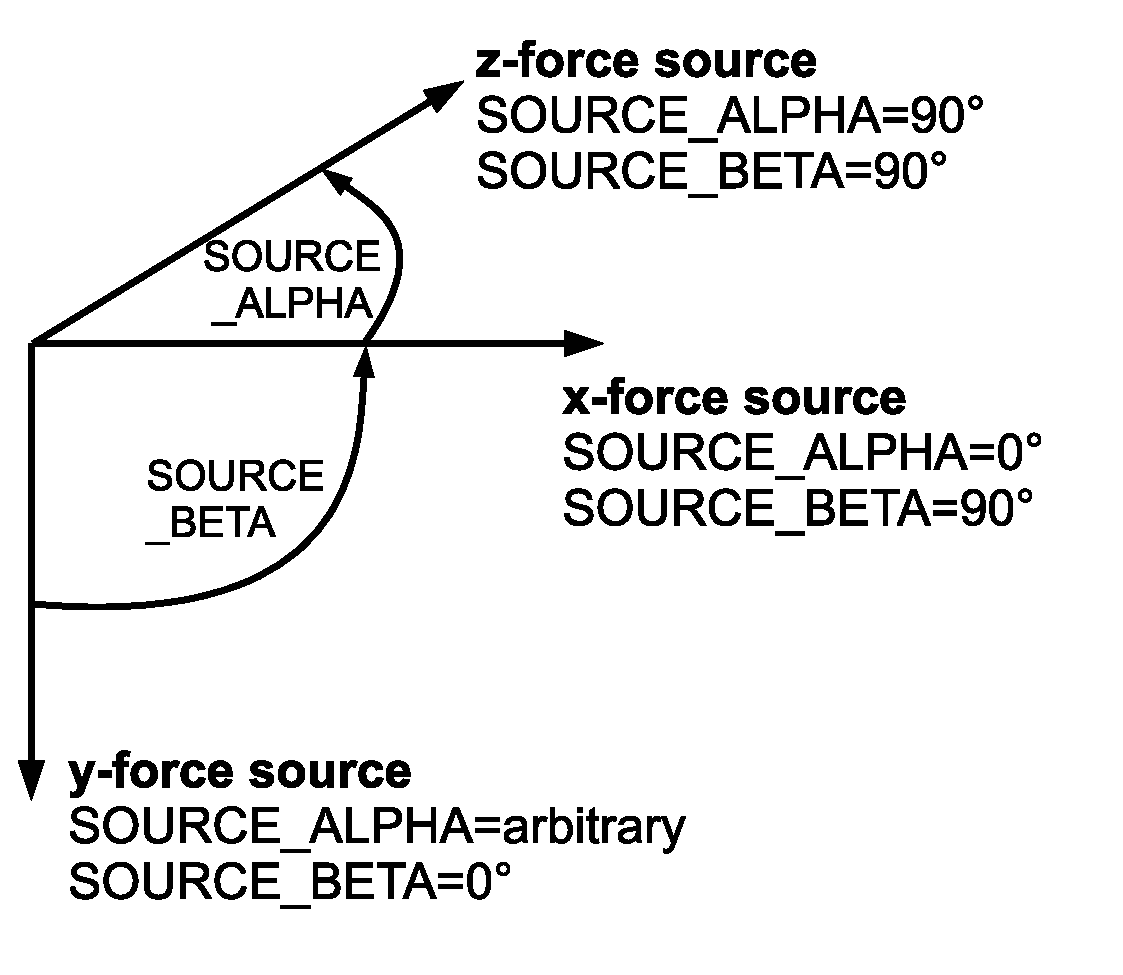
\includegraphics[width=7cm,angle=0]{eps/coordinate_system_customforcesource.pdf}
\end{center}
\caption{Scheme for SOURCE\_TYPE=5. The parameter SOURCE\_ALPHA denotes the angle between the horizontal x- and z-coordinate, while SOURCE\_BETA denotes the angle between horizontal x- and vertical y-coordinate. As an example, parameters for SOURCE\_ALPHA and SOURCE\_BETA are given in order to gain force sources in single coordinate direction (as specified by SOURCE\_TYPE=2-4)}
\label{coordinate_system_customforcesource}
\end{figure}


When using the earthquake double couple source (SOURCE\_TYPE=6), the orientation of the slip vector on the fault plane is defined by the angles STR, DIP and RAKE. For their definition see Figure \ref{Fig:EQS}. The earthquake source is implemented via a moment-tensor description \cite{graves:96}, while the moment-tensor components are derived from the strike, dip and rake angles \cite{aki:80}. The radiated energy of the earthquake is defined by the seismic moment, which is denoted by AMON. When using the earthquake double couple source output seismograms are in units of meters per second.

\tdplotsetmaincoords{0}{0}

\begin{figure}[h!]
\centering
\begin{tikzpicture}[scale=4]
\draw[thick,-stealth] (0,0,0) -- (1,0,0) node[anchor=west]{\textsf{\textbf{x East}}};
\draw[thick,-stealth] (0,0,0) -- (0,-1,0) node[anchor=west]{\textsf{\textbf{y Depth}}};
\draw[thick,-stealth] (0,0,0) -- (0,0,-1) node[anchor=south west]{\textsf{\textbf{z North}}};

\draw[-stealth,color=red] (0.35,-0.7,-0.75) -- (0.55,-0.35,-0.75);
\draw[dashed, color=red] (0,0,0) -- (0.1,-0.7,-0.5);
\draw[dashed, color=red] (0,0,0) -- (0.5,0,-0.5);
\draw[dashed, color=red] (0.5,0,-0.5) -- (0.6,-0.7,-1.0);
\draw[dashed, color=red] (0.1,-0.7,-0.5) -- (0.6,-0.7,-1.0);

\tdplotdrawarc{(0,0,0)}{0.4}{15}{45}{anchor=west}{\textsf{\textbf{STR}}};%$\phi$}
\tdplotdrawarc{(0.35,-0.7,-0.75)}{0.65}{33.5}{50.5}{anchor=west}{\textsf{\textbf{RAKE}}};%$\Lambda$}

\draw[dashed, color=black] (0.8,0,0.8) -- (-0.2,0,-0.2);
\draw[bend left=90] (0.1,-0.7,-0.5) -- (0.5,0,0.5) node[anchor=north west]{\textsf{\textbf{DIP}}};%$\delta$};
% \draw[thick,-stealth] (0.1,-0.69,-0.5) -- (0.1,-0.7,-0.5);

\end{tikzpicture}
\caption{The orientation of a simplified earthquake rupture plane is described by the strike angle STR, which is measured clockwise from north to the fault line, and the angle DIP, which denotes the angle between fault plane and the horizontal plane. The slip direction on the fault plane is denoted by the angle RAKE, which is measured counterclockwise from the horizontal fault line.}
\label{Fig:EQS}
\end{figure}



The locations of multiple sources must be defined in an external ASCII file (SOURCE\_FILE) that has the following format:
\begin{verbatim}
 %  XSRC        YSRC        ZSRC        TD      FC      AMP  
\end{verbatim}

More than one source position may be specified for example to simulate acoustic emission. In the following lines, you can define certain parameters for each source point:
XSRC is the x-coordinate of a source point (in meter), YSRC is the vertical y-coordinate of a source point (in meter), ZSRC is the horizontal z-coordinate of a source point (in meter).
TD is the excitation time (time-delay) for the source point [in seconds], FC is the center frequency of the source signal [in Hz], and AMP is the maximum amplitude of the source signal.

Please note that SOFI3D considers real physical units as input and output. AMP specifies a seismic moment of 1 Nm if an explosive source is chosen, in case of force source AMP specifies a force of 1 N. The seismogram output scales to this seismic moment or force and is given in particle velocities or pressure. Only the component \textit{div} and \textit{curl} cannot be treated as physical measures. For more information on the seismogram output see section \ref{Receivers}.

The  SOURCE\_FILE =  \lstinline{./sources/source.dat} that defines an explosive source  at $x_s=2592.0\;$ m, $y_s=2106.0\;$ m (depth) and $z_s=2592.0\;$ m  with no time delay,
a center frequency of 5 Hz  and an maximum amplitude of 1.0 reads, for example
\begin{verbatim}
    2592.0        2106.0        2592.0        0.0           5.0           1.0
\end{verbatim}

If the option RUN\_MULTIPLE\_SHOTS=0 in the parameter file all the shot points defined in the SOURCE\_FILE are used in one simulation. Setting RUN\_MULTIPLE\_SHOTS=1 will start model runs 
from i=1 to i=NSRC with source locations and properties defined at line i+1 of the SOURCE\_FILE. 

Instead of a single source or multiple sources specified in the SOURCE\_FILE, you can also specify to excite a plane wave parallel (or tilted by an angle PLANE\_WAVE\_ANGLE) to the top of the model. This plane wave is approximated by a plane of single sources at every grid point at a depth of PLANE\_WAVE\_DEPTH below. The center source frequency $f_c$ is specified by the inverse of the duration of the source signal TS. SOURCE\_SHAPE and SOURCE\_TYPE are taken from the parameters as described above. If you choose the plane wave option by specifying a PLANE\_WAVE\_DEPTH$>$0, the parameters SRCREC and SOURCE\_FILE will be ignored.

\subsection{Generation of models}
\label{gen_of_mod}
\begin{verbatim}
"Model" : "comment",
"READMOD" : "0",
"MFILE" : "model/test",
"WRITE_MODELFILES" : "0",

\end{verbatim}
READMOD : read model parameters from MFILE (yes=1) \\
READMOD = 1 -- binary files need to be provided
READMOD = 0 -- default parameters are generated by hh\_elastic on the fly, more models (hh\_elastic like files) can be found in src/hh\_old 
this was the recommended option for SOFI3D\\
READMOD = -1 -- halfspace with a layer with parameters specified in.json is generated by hh\_elastic. Parameters need to be specified in Tsvankin (1997) notation. DH1 specifies the depth at which the second layer is placed into the model and DH2 reflects its thickness.

\begin{verbatim}
"Model" : "comment",
"READMOD" : "-1",
"MFILE" : "model/test",
"WRITE_MODELFILES" : "0",

"VPV1"   : "1500.0",
"VSV1"   : "0.01",
"EPSX1"  : "0.0",
"EPSY1"  : "0.0",
"DELX1"  : "0.0",
"DELY1"  : "0.0",
"DELXY1" : "0.0",
"GAMX1"  : "0.0",
"GAMY1"  : "0.0",
"RHO1"   : "1000.0",
"DH1"    : "75",

"VPV2"   : "1800.0",
"VSV2"   : "500.0",
"EPSX2"  : "0.2",
"EPSY2"  : "0.1",
"DELX2"  : "0.05",
"DELY2"  : "0.2",
"DELXY2" : "-0.1",
"GAMX2"  : "0.15",
"GAMY2"  : "0.05",
"RHO2"   : "1560.0",
"DH2"     : "1000060.0",
\end{verbatim}
MFILE : String for the model file names, used to read from file and/or to write model for validation \\
WRITE\_MODELFILES : switch to decide whether all models RHO, U, Pi, Cij (and Taup, Taus) models (=1) or only the density model (=2) are written to file. In case of WRITE\_MODELFILES=0, no model file is written to file.

If READMOD=1, the P-wave, S-wave, Cij, and density model grids are read from external binary files. MFILE defines the basic file name that is expanded by the following extensions: P-wave model: ''.vp'', S-wave model: ''.vs'', density model: ''.rho''.  In the example above, the model files thus are: ''model/test.vp'' (P-wave velocity model),''model/test.vs'' (S-wave velocity model), and ''model/test.rho'' (density model). 

In these files, each material parameter value must be saved as 32 bit (4 byte) native float. Velocities must be in meter/second, density values in $kg/m^3$. The fast dimension is the y direction. See src/readmod.c. The number of samples for the entire model in the x-direction is NX, the number of values in the y-direction is always NY  and the number of values in the z-direction is always NZ. The file size of each model file thus must be NX*NY*NZ*4 bytes. You may check the model structure using the SU command ximage:

\lstinline {ximage n1=<NY> n2=<NX> < model/test.vp}.

If the variable TAU = 0.0 (see the next section \textit{Q-approximation}), it is also possible to read Qp, and Qs grid files to allow for spatial variable attenuation. In case of TAU > 0, constant damping is assumed with $Q_p=Q_s = \frac{2}{\mbox{TAU}}$. Please not that in order to ensure proper visualization using xmovie or ximage, the binary models are structured in terms of coordinate priority as follows : [Y,X,Z]. That means a 3-D model consits of NZ planes of the size NY $\times$ NX. The fast dimension of each NY-NX plane is the vertical Y-direction, i.e., first, columns of NY material parameters are written to file, in total NX columns of the length NY are written. To give an example of how to create a 3-D model using Matlab, the M-File  \lstinline{create_simple_tunnel_mod3D.m} is located in the folder  \lstinline{mfiles} (see Chapter \ref{installation}).

If READMOD=0 the model is generated ''on the fly'' by SOFI3D, i.e. it is generated internally before the time loop starts. We would prefer this way of generating the model grids because this way the size and the discretization intervals (DX, DY and DZ) can be controlled by the parameter file sofi3D.json. Furthermore, it is not necessary to generate (large) files by an external program. See section \ref{model_def_func} for an example function that generates the simple block model ''on the fly''. If READMOD=0 this function is called in sofi3D.c and therefore must be specified in src/Makefile (at the top of src/Makefile, see section \ref{compexec}). If you change this file, for example to change the model structure, you need to re-compile SOFI3D by changing to the src directory and ''make sofi3D''.

Due to the fact that the variable MFILE is also used to write the model - expanded by the extension-string ''SOFI3D'' to file for verification (also see the output file, section ''MODEL CREATION AND OUTPUT''), you can specify, whether only the density model is written (WRITE\_MODELFILES=0) or the Vp-velocity, Vs-velocity, density as well as Qp-damping and Qs-damping models (WRITE\_MODELFILES=1). BE AWARE that the output of additional models besides density cause extra but temporal memory allocation of the size of the local subgrid times the number of models! To give an example, the file name of the density models written for verification looks like this  \lstinline{model/test.SOFI3D.rho}.

\subsection{Q-approximation}
\begin{verbatim}
"Q-approximation" : "comment",
"L" : "0",
"FL1" : "5.0", 
"FREF" : "5.0",
"TAU" : "0.00001",
\end{verbatim}

with

L : Number of relaxation mechanisms\\
FL1 : First relaxation frequency \\
FREF : Reference frequency where no velocity dispersion occurs \\
TAU : TAU value for entire model\\

These lines may be used to define an overall level of intrinsic (viscoelastic) attenuation of seismic waves, i.e. a constant (spatially not varying) TAU = 2/Q for the complete model. The level of attenuation is defined by Q. Note that small Q values ($Q<50$) may lead to significant amplitude decay and velocity dispersion. The relaxation frequency (FL1) can be specified to approximate the constant Q for all frequencies. The frequency dependence on attenuation, i.e., Q and phase velocity as a function  of frequency, may be calculated using the Matlab functions in the directory mfiles.
In the current version, only one (so-called) relaxation mechanism (L=1) is implemented \cite{bohlen:98,blanch:95,bohlen:02}. The possible values for L thus are L=1 and L=0. In case of L=0, a purely elastic simulation is performed (no absorption). In the elastic case (L=0), the memory requirements and run time of the program are reduced by approximately 30 per cent. The parameter FREF determines the frequency where no velocity dispersion occurs. Generally, FREF equals the largest center frequency FC of sources defined in SOURCE\_FILE. In fact, if FREF is not specified or set to 0.0, FC is used instead.

If you set TAU=0.0, it is further possible to simulate any spatial distribution of absorption by assigning the gridpoints with different Q-values by reading external grid files for Qp (P-waves) and Qs (S-waves) (see src/readmod.c) or by generating these files ''on the fly'' (see section \ref{model_def_func}). If TAU$>$0.0 no external Qp and Qs-file will be read in, instead TAU will be used for a constant Q-model.

Please note, that due to dispersive media properties the viscoelastic velocity model is only defined for the reference frequency only. In sofi3D, this reference frequency is specified as the center source frequency. At the exact reference frequency, elastic and viscoelastic models are equivalent. As a consequence, slightly smaller and larger minimum and maximum velocity values occur in the viscoelastic model.


\subsection{Boundary conditions}
\label{abs}

\begin{verbatim}
"Boundary Conditions" : "comment",
    "FREE_SURF"  : "1",
    "ABS_TYPE"   : "2",
    "FW"         : "30.0",
    "DAMPING"    : "8.0",
    "FPML"       : "5.0",
    "VPPML"      : "3500.0",
    "NPOWER"     : "2.0",
    "K_MAX_CPML" : "10.0",
    "BOUNDARY"   : "0",
\end{verbatim}
where\\
\option{FREE\_SURF}: free surface (no=1; yes=1)\\
\option{ABS\_TYPE}: type of boundary condition (Convolutional Perfectly Matched Layer (CPML)=11; exponential damping=2)\\
\option{FW}: width of the absorbing boundary frame (in grid points) (the frame is absent when \option{FW$\leq$0})\\
\option{DAMPING}: percentage of amplitude decay at the outer edge, applied when (\option{ABS\_TYPE=2})\\
\option{FPML}: dominant frequency (in Hz), applied for CPML (when \option{ABS\_TYPE=1})\\
\option{VPPML}: $p$-wave velocity near the boundary (in m/s), applied for CPML (when \option{ABS\_TYPE=1})\\
\option{NPOWER}:  exponent used for CMPL (when \option{ABS\_TYPE=1}), the larger \option{NPOWER} the more damping \\
\option{K\_MAX\_CPML}:  coefficient applied for CPML (when \option{ABS\_TYPE=1}) \\
\option{BOUNDARY}: apply periodic boundary condition at edges (no=0;
left/right/front/back/top/bottom=1)
%A : thickness of the layer between aquisition geometry and PML \\

The boundary conditions are applied on each side face and the bottom face of
the model grid. If \option{FREE\_SURF=1}, then a plane stress free surface is
applied at the top of the global grid  using the imaging method proposed by
Levander~\cite{levander:88}, otherwise the specified boundary condition is also
applied at the top face of the model grid. Note that the absorbing frame is
always located INSIDE the model space, i.\ e., parts of the model structure are
covered by the absorbing frame, in which no physically meaningful wave
propagates. You should therefore consider the frame width when you design the
model structure and the acquisition geometry (shot and receivers should
certainly be placed outside).

Two different absorbing boundary conditions are available: an unsplit
convolutional perfectly matched layer (CPML) boundary condition (in the elastic
case) and split perfectly matched layer (PML) boundary condition (in the
acoustic case), respectively, and a conventional exponential wavefield damping
condition (ABS) (see Section~\ref{bound_cond}).

If \option{ABS\_TYPE=1}, the PML implementation is based on the papers
\cite{collino:01,komatitsch:07,martin:09}. It should be
much more effective than the ABS condition. A width of the absorbing frame
\option{FW} of 10--20 grid points should be sufficient. For the optimal
realization of the CPML boundary condition you have to specify the dominant
signal frequency \option{FMPL} occurring during the wave simulation. This is
usually the center source frequency \option{FC} specified in the source file.
\option{VPPML} should be approximately the $p$-wave velocity near the model
boundaries. For the definition of the option \option{VPPML}, have a look at
$V_p$ in equation \ER{FD:6:1}. If the wave incident angle is not perpendicular
to CPML frame, \option{K\_MAX\_CPML} can be increased in order to stabilize the
CPML update, otherwise instabilities might occur.

If \option{ABS\_TYPE=2}, then exponential wavefield damping is applied on the
boundaries according to~\cite{cerjan:85}. For this case, the width of the frame
(\option{FW}) should be at least 30--50 grid points. \option{DAMPING} specifies
attenuation in percent at the edges of the numerical grid, i.\ e., amplitudes
are multiplied by a factor of 1-DAMPING at the outer edges. A good choice for
\option{DAMPING} is 8 \%. For larger values, reflections at the onset of the
absorbing frame might occur. In order to avoid such an impedance contrast
between the model domain and the absorbing boundary frame, you may as well
increase \option{FW} and decrease \option{DAMPING}.

It is sometimes useful to apply periodic boundary conditions (see
Section~\ref{bound_cond}). If \texttt{BOUNDARY=1}, no absorbing boundaries are
installed at the left/right, front/back, and top/bottom sides of the grid.
Instead, wavefield information is copied from left to right and vice versa,
etc. The effect is that a wave which, for example, leaves the model at the left
side, enters the model again at the right side.

\subsection{Wavefield snapshots}
\begin{verbatim}
"Snapshots" : "comment",
"SNAP" : "4",
"TSNAP1" : "6.6e-3",
"TSNAP2" : "4.8",
"TSNAPINC" : "0.2",
"IDX" : "1",
"IDY" : "1",
"IDZ" : "1",
"SNAP_FORMAT" : "3",
"SNAP_FILE" : "./snap/test",
"SNAP_PLANE" : "1",
\end{verbatim}

with

SNAP : output of snapshots (yes$>$0) (particle-velocities=1, pressure field=2, curl and divergence energy=3, particle velocities and energy=4)\\
TSNAP1 : first snapshot (in sec)\\
TSNAP2 : last snapshot (in sec)\\
TSNAPINC : increment (in sec)\\
Note that Y denotes the vertical direction!\\
IDX : increment x-direction (in grid points)\\
IDY : increment y-direction (in grid points)\\
IDZ : increment z-direction (in grid points)\\
SNAP\_FORMAT : data-format (ASCII(2);BINARY(3))\\
SNAP\_FILE : basic filename, the output will look like SNAP\_FILE.bin.z.000, if SNAP = 1,2 SNAP\_PLANE is ignored\\
SNAP\_PLANE : output of snapshots as energy (without sign=1, with sign true for x-z-plane=2, with sign true for x-y-plane=3, with sign true for y-z-plane=4)\\


If SNAP$>0$, wavefield information (particle velocities, pressure, or curl and divergence of particle velocities) for the entire model is saved on the hard disk (assure that enough free space is on disk!). Each PE is writing his sub-volume to disk. The filenames have the basic filename SNAP\_FILE plus an extension that indicates the PE number in the logical processor array (see Figure \ref{fig_grid}), i.e. the PE with number PEno writes his wavefield to SNAPFILE.PEno. The first snapshot is written at TSNAP1 seconds of seismic wave traveltime to the output files, the second at TSNAP1+TSNAPINC seconds etc. The last snapshots contains wavefield at TSNAP2 seconds. Note that the file sizes increase during the simulation. The snapshot files might become quite LARGE. It may therefore be necessary to reduce the amount of snapshot data by increasing IDX, IDY and IDZ and/or TSNAPINC. A detailed description how to visualize 3-D wavefields is given in section \ref{visual}. In order to merge the separate snapshot of each PE after the comletion of the wave modeling, you can use the program snapmerge (see Chapter \ref{installation}, section \textbf{src}). The bash command line to merge the snapshot files can look like this:  \lstinline{../bin/snapmerge ./in_and_out/sofi3D.json}.

\subsection{Receivers}
\label{Receivers}
\begin{verbatim}
"Receiver" : "comment",
"SEISMO" : "4",
"READREC" : "0",
"REC_FILE" : "./receiver/receiver.dat",
"REFRECX, REFRECY, REFRECZ" : "0.0 , 0.0 , 0.0",
"XREC1,YREC1, ZREC1" : "54.0 , 2106.0, 2592.0",
"XREC2,YREC2, ZREC2" : "5400.0 , 2106.0, 2592.0",
"NGEOPH" : "1",
\end{verbatim}

with 

SEISMO : output of seismograms (no seismograms=0, particle-velocities=1, pressure (hydrophones)=2, curl and div=3, everything=4)\\
READREC : read receiver positions from file (yes=1)\\
REC\_FILE : external receiver file name\\
REFREC : reference point for receiver coordinate system\\
if READREC=1 the REC1,YREC1,ZREC1, XREC2,YREC2,ZREC2 and NGEOPH are ignored\\ 
REC1,YREC1,ZREC1 : position of first receiver (in m)\\
XREC2,YREC2,ZREC2 : position of last receiver (in m)\\
NGEOPH : distance between two adjacent receivers (in gridpoints)\\


If SEISMO$>$0, seismograms are saved on hard disk. If SEISMO equals 1 x-, y-, and z-component of particle velocity will be written according to parameters specified in Chapter \ref{seismograms}.
If SEISMO==2 pressure (sum of the diagonal components of the stress tensor) recorded at the receiver locations (receivers are hydrophones!) is written. if SEISMO=3 the curl and divergence are saved. As described in section \ref{Sources} the seismogram output is physically correct for a seismic moment of 1 Nm (explosive source) and a force of 1 N (force source), respectively.

The curl and divergence of the particle velocities are useful to separate between P- and S-waves in the snapshots of the wavefield. SOFI3D calculates the divergence and the magnitude of the curl of the particle velocity field \cite{dougherty:88}. The motivation for this is as follows. According to Morse and Feshbach \shortcite{morse:53} the energy of P- and S-wave particle velocities is, respectively,
\begin{equation}
E_p=\left(\lambda + 2 \mu\right) (div(\vec{v}))^2 \quad \mbox{and} \quad E_s=\mu \left|rot(\vec{v})\right|^2 \quad\mbox{.}
\label{eq_E}
\end{equation}
$\lambda$ and $\mu$ are the Lam\`{e} parameters, and $\vec{v}$ is the particle velocity vector. In order to preserve the divergence and curl sign information  while showing relative compressional
and shear particle velocity amplitudes, we plot the following quantities:
\begin{equation}
\bar{E}_p=sign(div \vec{v}) E_p^{1/2} \quad \mbox{and} \quad \bar{E}_s= sign(rot\vec{v}) E_s^{1/2} \quad\mbox{,}
\label{eq_e}
\end{equation}
The magnitudes of $\bar{E}_p$ and $\bar{E}_s$ are proportional to the magnitudes of the P- and S- particle velocities, respectively. Note that interface waves like Rayleigh waves contain both a P- and S-wave component and therefore show up on both quantities of equation \ref{eq_e}.

The locations of the receivers may either be specified in a separate file REC\_FILE or in this parameter file. If READREC=1 receiver locations are read from the ASCII-file REC\_FILE. Each line contains the coordinates of one receiver, the first two number in each line indicate the horizontal x-coordinate, the vertical y-coordinate and the third number denotes the horizontal z-coordinate of each receiver position. To give an example of a receiver file, the following 3 lines specify 3 receivers located at constant depth (2106.0 m) and horizontal y-coordinate (2592.0 m). However, the receiver coordinates change in x-direction (starting at 540 m) and therefore lining up along the x-axis.  
\begin{verbatim}
540.0   2106.0   2592.0   
1080.0  2106.0   2592.0
1620.0  2106.0   2592.0
\end{verbatim}
These receiver coordinates in REC\_FILE are shifted by REFREC[1], REFREC[2] and REFREC[3] into the  x-, y- and z-direction, respectively. This allows for completely moving the receiver spread without modifying REC\_FILE. This may be useful for the simulation of moving profiles in reflection seismics.

If READREC=0 the receiver locations must be specified in the parameter file. In this case, it is assumed that the receivers are located along a straight line. The first receiver position is defined by (XREC1, YREC1, ZREC1), and the last receiver position by (XREC1, YREC1, ZREC1) (see Figure \ref{fig_grid}). The spacing between receivers is NGEOPH grid points.  A Vertical Seismic Profile (VSP)
is realized when XREC1=XREC2, YREC1$<$YREC2.  

Receivers are always located on full grid indices, i.e. a receiver that is located between two grid points will be shifted by the FD program to the closest next grid point. It is not yet possible
to output seismograms for arbitrary receiver locations since this would require a certain wavefield interpolation.

\textbf{It is important to note that the actual receiver positions defined in REC\_FILE or in sofi3D.json may vary by DX/2 and/or DY/2 and/or DZ/2 due to the staggered positions of the particle velocities and stress tensor components. }

In our example, we specify 100 receiver location. Due to the small size of the model, most of the specified receiver positions will be located inside this absorbing boundary (if ABS=2, see Chapter \ref{abs}). A corresponding warning message will appear. If you choose to read the receiver location from REC\_FILE  \lstinline{./receiver/receiver.dat} (READREC=1), only 10 receivers locations are considered. The list of receivers specified in file  \lstinline{./receiver/receiver.dat} is equivalent to the parameters in the input file with only a larger distance between adjacent receivers (NGEOPH = 10.)

\subsection{Receiver array}
\begin{verbatim}
"Receiver array" : "comment",

"REC_ARRAY" : "0",
"REC_ARRAY_DEPTH" : "1350.0",
"REC_ARRAY_DIST" : "640.0", 
"DRX" : "2",
"DRZ" : "2",
\end{verbatim}

A horizontal 2-D array of receivers is simulated if REC\_ARRAY$>$0. This option specifies the number of receiver planes horizontal to the x-z-plane (surface of the model). The first plane is located in depth REC\_ARRAY\_DEPTH meter. The second plane in REC\_ARRAY\_DEPTH + REC\_ARRAY\_DIST, the last in REC\_ARRAY\_DEPTH + (REC\_ARRAY-1) $\times$ REC\_ARRAY\_DIST. The distance between receivers within each plane is DRX and DRZ grid points (DRX*DX and DRZ*DZ meters).

\subsection{Seismograms}
\label{seismograms}
\begin{verbatim}
"Seismograms" : "comment",
"NDT, NDTSHIFT" : "1, 0",
"SEIS_FORMAT" : "1",
"SEIS_FILE" : "./su/test",
\end{verbatim}

with

NDT, NDTSHIFT : samplingrate and timelag (in timesteps!). Write every (NDT)th sample, leaving NDTSHIFT samples at the beginning out\\
default: NDT=1 and NDTSHIFT=0. (NDT=0 is set to NDT=1, NDT$<$0 are set to -NDT.)\\
caution: previous versions used NDTSHIFT=NDT-1\\
SEIS\_FORMAT : data-format, values:
\par
\begingroup
\leftskip=0.5cm
0 = SEG-Y (ASCII-text/native 4-byte-floats (IEEE on PC)/little endian on PC)\\
1 = SU (native 4-byte-floats (IEEE on PC)/little endian on PC)\\
2 = TEXTUAL (native ASCII)\\
3 = BINARY (IEEE-4-byte-floats on PC/little endian on PC)\\
4 = SEG-Y (ASCII-text/native 4-byte-floats (IEEE on PC)/little endian on PC)\\
5 = SEG-Y (ASCII-text/IBM-4-byte-floats on PC/big endian on PC) \\
\par
\endgroup
SEIS\_FILE : basic filename according to output\_ of\_seismograms (SEISMO), separate seismogram files are outputted and will look like  \lstinline{SEIS_FILE_vz.su} or  \lstinline{SEIS_FILE_div.segy}.

If SEISMO$>$0 seismograms recorded at the receiver positions are written to the corresponding output files. The sampling rate of the seismograms is NDT*DT seconds. In case of a small
time step interval and a high number of time steps, it might be useful to choose a high NDT in order to avoid a unnecessary detailed sampling of the seismograms and consequently large files of seismogram data. Possible output formats of the seismograms are SU, ASCII, BINARY, SEGYa or SEGYe. It is recommended to use SU format as seismogram output. The main advantage of this format is that the
time step interval (NDT*DT) and the acquisition geometry (shot and receiver locations) are stored in the corresponding SU header words. Also, additional header words like offset are set by SOFI3D. This format thus facilitates a further visualization and processing of the synthetic seismograms.

Note, however, that SU cannot handle sampling rates smaller than 1.0e-6 seconds and the number of samples is limited to about 32.000. In such cases, you should increase the sampling rate by increasing NDT. If this is impossible (for example because the Nyquist criterion is violated) you must choose a different output format (ASCII or binary).

Each PE internally stores seismograms which are recorded in his portion of the grid. After finishing the time step loop, the seismogram parts are internally exchanged and the merged seismograms are collectively saved to file. The filenames are expanded according to basic file name SEIS\_FILE and the SEISMO option (pressure, particle velocity, curl, divergence). To give an example, PE0 writes the merged seismograms of the x-component of particle velocity to  \lstinline{SEIS_FILE_vx.su} if the output is chosen to be according to the SU file format. 

%If SU-files are output these can be merged together by using the Unix command cat. For example to merge seismograms of the vx-component of particle velocity into one single SU-file use:
%\emph{cat SEIS\_FILE\_VR.* $>$ SEIS\_FILE\_VR} 
%The shell script  \lstinline{sucat.sh} merges all seismograms at the same time.

\subsection{Monitoring the simulation}
\begin{verbatim}
"Monitoring the simulation" : "comment",
"LOG_FILE" : "log/test.log",
"LOG" : "1",
"OUT_SOURCE_WAVELET" : "0",
"OUT_TIMESTEP_INFO" : "10",

\end{verbatim}

with

LOG: output of logging information of node (no output=0; to stdout=1; to file LOG\_FILE=2)\\
LOG\_FILE : log-file for information about progress of program (each PE is printing log-information to LOG\_FILE.MYID) \\
OUT\_SOURCE\_WAVELET : output of used source wavelet (yes=1/no=0) \\
OUT\_TIMESTEP\_INFO : every OUTNTIMESTEPINFOth time step information on update and exchange times are written in LOG\_FILE 


SOFI3D can output a lot of useful and possibly not useful information about the modeling parameters and the status of the modeling process etc. The major part of this information is output by PE 0.
If LOG=1, PE 0 writes this info to stdout, i.e. on the screen of your shell. This is generally recommended  to monitor the modeling process. You may want to save this screen info to a output file by adding  \lstinline{> sofi3D.jout} or  \lstinline{|tee sofi3D.jout}. to your starting command. If LOG=1 all other processes with PE number (PEno) greater than zero will write their information to LOG\_FILE.PEno. If you specify LOG=2 also PE 0 will output his information to LOG\_FILE.0. As a consequence only little information is written directly to the screen of your shell. On supercomputers where you submit modeling jobs to a queuing system as batch jobs LOG=2 may be advantageous. In case of LOG=2, you may still watch the simulation by checking the content of LOG\_FILE.0 for example by using the Unix commands more or tail. After finishing the program the timing information is written to the ASCII file log/test.log.0.timings. If LOG=0 no output from node 0 will be written, neither to stdout nor to an LOG file. There will be also no output of timing information to the ASCII file log/test.log.0.timings. 

By using the switch OUT\_SOURCE\_WAVELET you can decide to output the used source wavelet (yes=1/no=0). Every PE that includes a source locatation will than outputs the source signal time series as SU output. Due to the fact that the output of information on the update and exchange via fprint can be both slowing down the computation for very small models and producing large output files, you can choose by OUT\_TIMESTEP\_INFO after how many time steps such intermediate information are given.

\subsection{Checkpointing}
\begin{verbatim}
"Checkpoints" : "comment",
"CHECKPTREAD" : "0",
"CHECKPTWRITE" : "0",
"CHECKPT_FILE" : "tmp/checkpoint_sofi3D",
\end{verbatim}

with 

CHECKPTREAD : read wavefield from checkpoint file (yes=1/no=0)\\
CHECKPTWRITE : save wavefield to checkpoint file (yes=1/no=0)\\
CHECKPTFILE : checkpoint file name\\

On most supercomputers with a queuing system the run time of job is limited. Sometimes the allowed run time is not sufficient to finish a FD simulation. In such a case, check-pointing can be performed: the first job saves the complete elastic wavefield (CHECKPTWRITE=1) but does not! read the wavefield from a checkpoint file (CHECKPTREAD=0). The subsequent jobs read and write the wavefield to the CHECKPTFILE, i.e. CHECKPTREAD=1 and CHECKPTWRITE=1. In this manner, one simulation can be divided on different batch jobs. The resulting seismograms may be catenated using the SU-command suvcat. But be aware that the checkpointing option saves the COMPLETE wavefield information of the last time step, which can produce a huge amount of data.

\subsection{''On the fly'' definition of material parameters}
\label{model_def_func}
If you choose to create the model ``on the fly'', the distribution of the
material parameters P-wave velocity $v_p$, S-wave velocity $v-s$ and density
$\rho$ for the simple block model has to be defined in the function hh.c that
can be found in the src folder. While ``programming'' the model, please note
the orientation of the coordinate system (see Chapter \ref{coord_system} for
more information). An example C-file ( \lstinline{src/model_elastic.c}) for the
generation of an elastic model is given in the following:

%\VerbatimInput{../../src/model_elastic.c}

As you can see from lines
\begin{verbatim}
    sprintf(modfile,"%s.mod",MFILE);
    writemod(modfile,rho,3);
\end{verbatim}
the density model is written to file to be displayed as described in Chapter \ref{gen_of_mod}. As a base name for the model file, the variable MFILE from the input file is used that actually specifies the external velocity and density files. Note, that the thickness of the first layer \textit{h} is set to 10000 m (10km) which is larger than the vertical extension (NY*DH=5400 m). This way, we effectively created a homogeneous model while demonstrating a two layer case. Simple decrease the variable \textit{h} to 2700 and a real two layer model is created. Generally, you only have to modify the material property definitions in the upper part of the model file and code some if statements to construct simple structures such as planes, cubes, tubes, etc.

\subsection{Compilation of SOFI3D}\label{compexec}
The source codes are located in the directory src. To compile SOFI3D the name of the model function has to be entered in the MAKEFILE. Depending on your MPI environment (MPI distribution) you may need to modify the compiler options in src/Makefile. For a few typical platforms the compiler options are available in src/Makefile. It is often usefull to enable the highest level of optimization (typically -03 or -04). No other changes in the Makefile should be necessary. 
\begin{verbatim}
# Makefile for SOFI3D 

#--------------------------------------------------------
# edit here

# source code for model generation (viscoelastic)
MODEL_SRC_V = model_visco.c

# source code for model generation (elastic)
MODEL_SRC_E = model_elastic.c

# source code for model generation (acoustic)
MODEL_SRC_A = model_acoustic.c

# source code for benchmark model
MODEL_SRC_BENCH = benchmod.c

# Compiler (LAM: CC=hcc, CRAY T3E: CC=cc, SHARCNet: mpicc)

# On Linux cluster running LAM
# CC=hcc
# LFLAGS=-lm -lmpi
# CFLAGS=-g -Wall -O4

# On CRAY T3E
# CC=cc

# On Linux Cluster using OpenMPI
 CC=mpicc
 LFLAGS=-lm
 CFLAGS=-Wall -O3

# On InstitutsCluster2 using intelMPI AND ITAC (no optimization)
# CC = mpicc
# LFLAGS = -tcollect
# CFLAGS = -tcollect -trace

# On InstitutsCluster2 using Open MPI and scalasca (no optimization)
#CC = skin mpicc
#LFLAGS =
#CFLAGS =-O3

#On InstitutsCluster2 using Open MPI and DDT (no optimization)
#CC = mpicc
#LFLAGS = -g
#CFLAGS = -g -O0 -i_dynamic


# On JUROPA cluster
#CC=mpicc
#LFLAGS=-lm
#CFLAGS=-O3 -ipo 


# On HLRN system
#CC=mpcc
#LFLAGS=-lm  

# ON Linux cluster ALTIX.RZ.UNI-KIEL:DE
#CC=icc
#CFLAGS=-mp -O3 -ip0q
#LFLAGS=-lmpi -lm

# ON Linux cluster ALTIX.HRZ.TU-FREIBERG.DE
#CC=icc
#CFLAGS=-mp -O3 -ip0
#LFLAGS=-lmpi -lm -i-static


# after this line, no further editing should be necessary
# --------------------------------------------------------
\end{verbatim} 
To compile the program SOFI3D you must change to the  \lstinline{src} directory and execute:
 \lstinline{make all}
or
 \lstinline{make sofi3D}
The program snapmerge that is used to merge the snapshots (see below) can be compiled with ''make snapmerge''. Since this is not a MPI program (no MPI functions are called) the MPI libraries are not required and any standard compiler (like gcc and cc) can be used to compile this program. The executables sofi3D and snapmerge are located the directory bin.

\subsection*{Running the program}
We recommend to create clones of the par folder for individual simulations. All the code inputs and outputs are then contained within those folders.

\section{Visualization with MATLAB} \label{visual}
Inside mfiles folder you will find the following scripts:
\begin{verbatim}
merge_snapshots.m
read_asofi3D_json.m
snap3D_ASOFI.m.
\end{verbatim}
Run snap3D\_ASOFI.m to visualize the snapshots. You should get smth like this
\begin{figure}[ht]
	\centering
	
	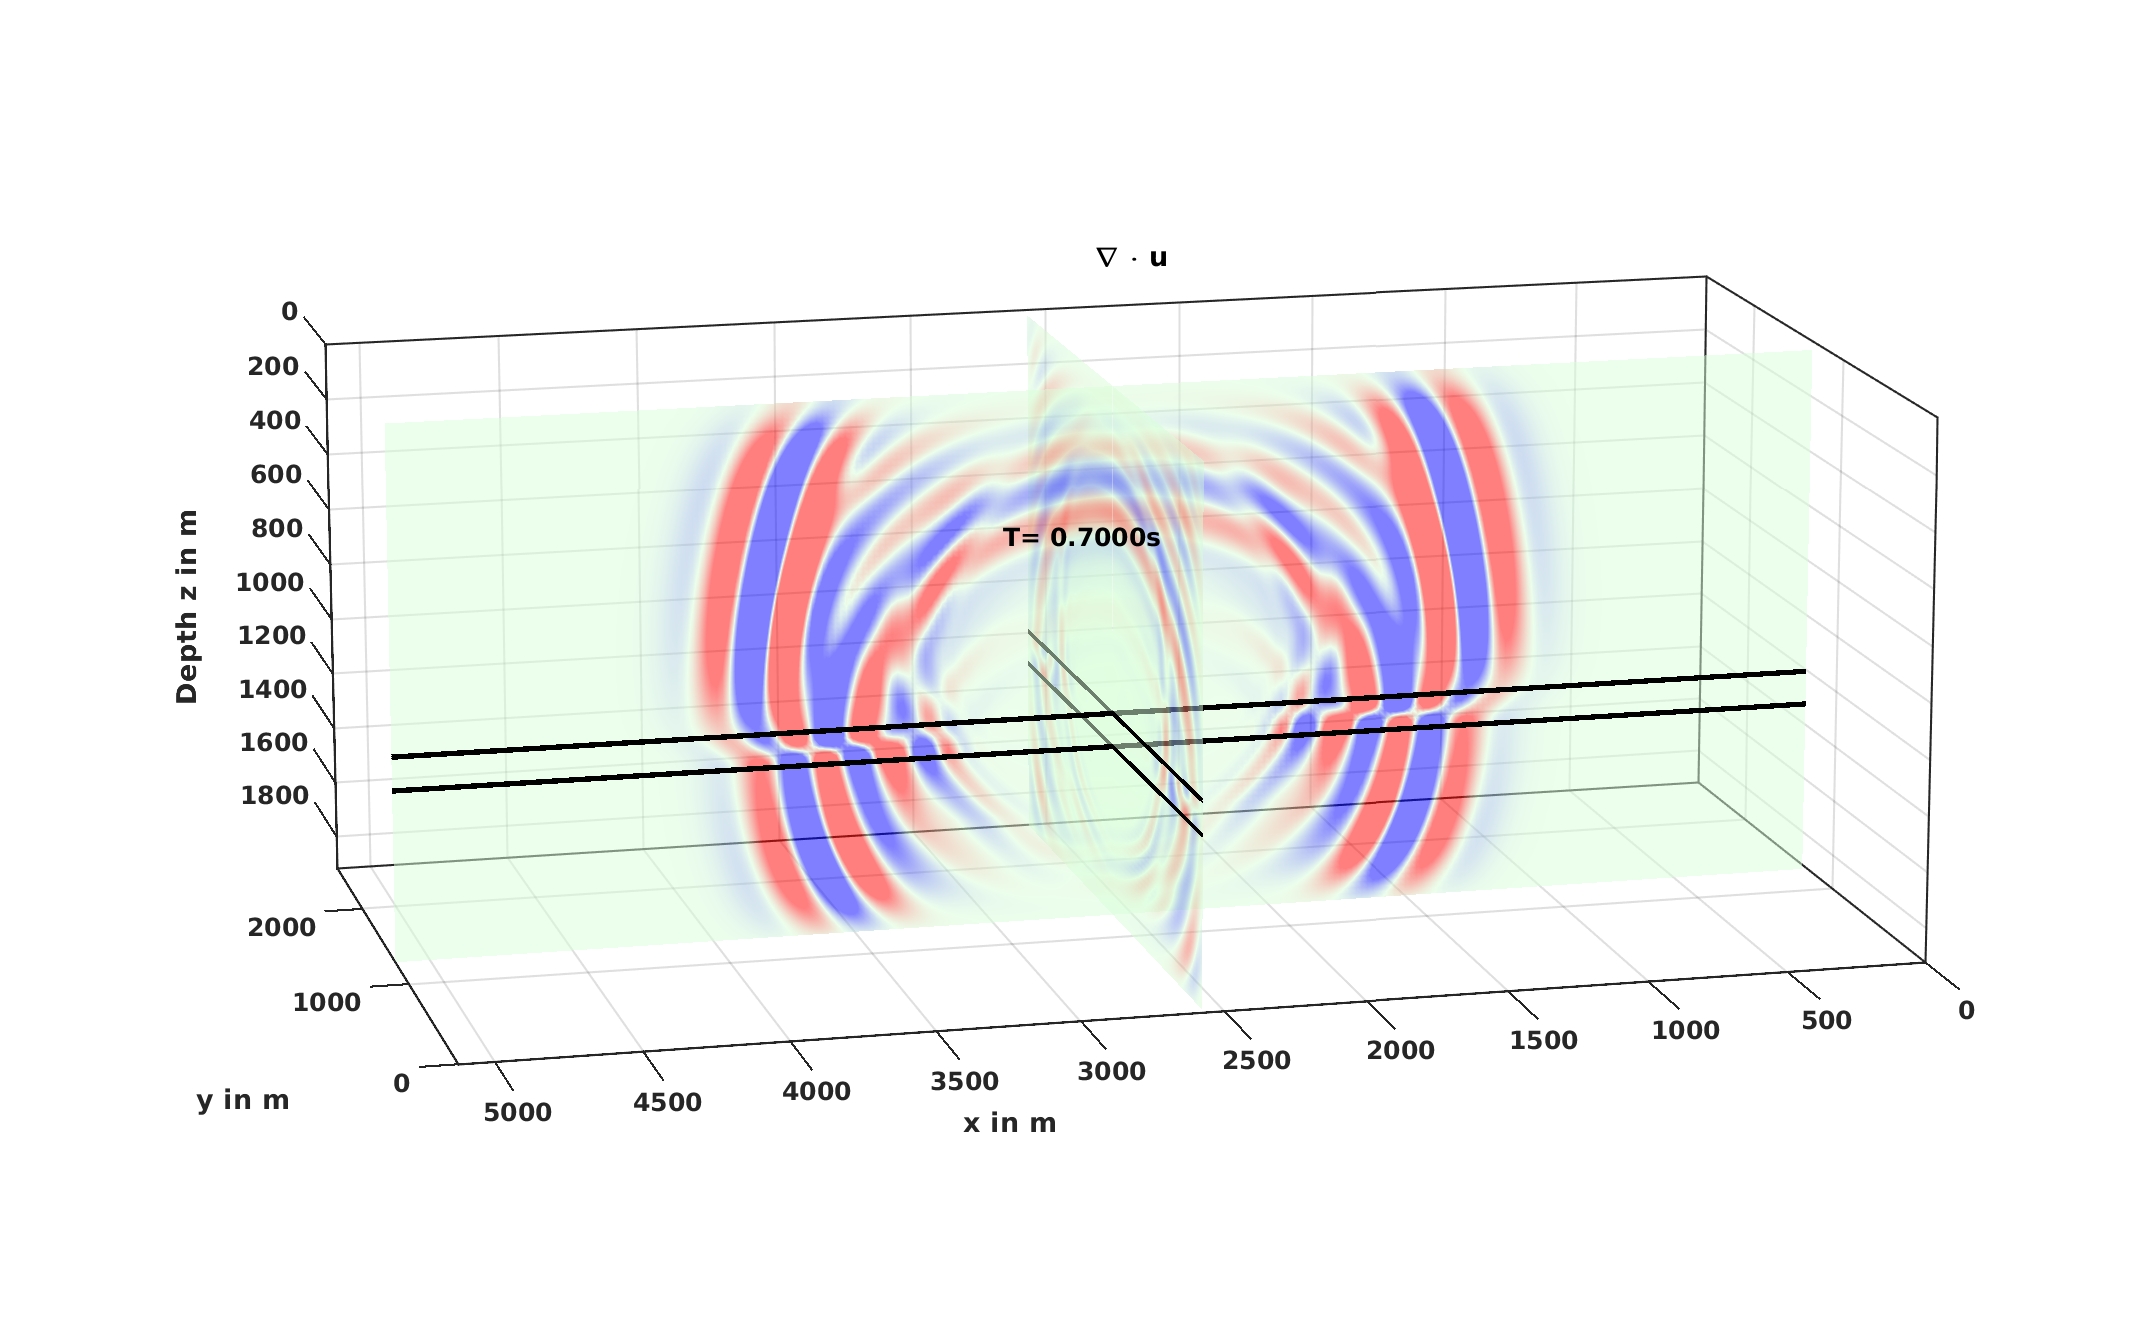
\includegraphics[width=0.9\linewidth]{eps/defaultSnap}
	\caption{Wave propagation in anisotropic medium. Snapshot is produced with default parameter file}
	\label{fig:defaultSnap}
\end{figure}
merge\_snapshots.m, can help you merge snapshots faster than bin/snapmerge, if they fit into the RAM of your workstation.

\newpage
\section{Acknowledgments}

We thank KAUST for support and KSL for computational resources to test the code. We are also grateful to Thomas Bohlen and his team from KIT, who released isotropic SOFI3D, which we based our development on. Finally, we would like to thank Tariq Alkhalifah and Seismic Wave Analysis Group (SWAG) for discussions and comments on the code. We also validated the code with recent normal mode theory \cite{ivanov2018} and thank Alexey Stovas and Yuriy Ivanov of NTNU for their contribution to that. Juwon Oh and Mahesh Kalita we thank, in particular, for their direct contributions to the code development. For full list of developers have a look at the file ``AUTHORS".







 





\bibliography{thesis}
\end{document}
\grid
\grid
